\chapter{Portfolio optimisation}
\graphicspath{{Chapter4/figures/}}
\label{lab:PO}
Optimal portfolio is the ultimate goal of every investment manager; but the optimality criteria can be very different to each of them. In the infamous Markowitz's modern portfolio theory \cite{HM52}. it is assumed that investor attempt to maximize a portfolio's return and minimize the risk (measured by the variance of the portfolio return). For index tracker fund manager, the main objective of portfolio management is to track and replicate the exposure of a benchmark index. The lack of active management generally makes the fund less vulnerable to change of management and has the advatanges of lower fees and taxes. It is the latter the focus of the thesis lies.
 
This chapter begins with a brief introduction on index tracking fund and a short summary on some causing factors of the tracking error between a index fund and its benchmark index. It then describes how the portfolio optimisation problem in terms of minimising the tracking error can be formulated as a stochastic control problem, which is then turned into a parameter estimation in the SMC framework. Next, it details some of the experiments carried out to verify this approach, starting with a simple proof of concept experiment in Section \ref{sec:exp1}, continue on with a more complicated example with real-world data in Section \ref{sec:exp2} and concludes the chapter with an experiment in demonstrating how the Model Predictive Control (MPC) can be incorporating into the basic SMC framework proposed.
 
%We investigate in this chapter how SMCs can be used to search for the optimal control parameters for portfolio optimisation problem in financial market, i.e., what decision a portfolio manager need to do to minimize the portfolio's tracking error to the target's stock index over a finite time horizon. This chapter is organised as follows: In Section \ref{sec:po}  shows how a portfolio optimisation problem can be re-casted into a parameter estimation problem in SMC framework. Section \ref{sec:toy} details the experiments in accessing how well this approach perform to track various target signals generated by some known models. Section \ref{sec:real} presents the experiments of examining the approach using real-world data collected from Yahoo finance. Section \ref{sec:extension} details possible extensions that can be easily achieved with this framework with some concrete examples. Finally, Section \ref{sec:summary} concludes this chapter with a summary of results.
 
\section{Index Tracking Fund}
An financial index can be thought of a summary statistics of a market, typically formed as weighted average of the prices of some financial instruments. For example, FTSE 100 is an index that attempts to represents the performance of the 100 biggest companies in UK. This index is however not an investable financial product one can invest directly.
 
To allows investors to take exposure to the markets (as represented by the indices), index tracker funds are introduced. These funds generally follow very strict and transparent rules with the main objective to track their benchmark indices as close as possible. Investors of these funds therefore are only exposed to the market risks of the chosen indices, with minimal exposure to the risk associated with the investment process of the traditional active fund management.
 
\subsection{Index Replication}
To track an index, the simplest way is to replicate the index by investing all the components of the benchmark index. However, this can be costly and difficult to manage, considering some of the indices may have huge number of components, e.g., MSCI World index that consists of $\approx 1600$ components from many different countries. Instead, one could partial replicate the index by sampling some of the components that are most representative. This can mean those components with larger weights, more volatiles or less correlated in returns (assuming these returns average out the gain/loss among them). This partial replication could save transaction cost, at the same time, introducing some tracking errors to the funds.
 
Instead of physically replicating the index by investing in the components, the portfolio manager also have the option to enter a swap agreement with a counterparty (typically investment bank) that provides the exact return of the stock market or commodity it’s tracking. Essentially, this transfers the market risk to the counterparty, at the same introducing the counterparty default risk. This technique is known synthetic replication.
 
\subsection{Causing factors of tracking error}
To evaluate the performance of index tracking fund, different metrics have been introduced to quantify the mismatch between the performance of a fund and its benchmark index. For example, tracking difference is the sum of absolute difference in returns between of a fund and its benchmark. Here, we adopt the tracking error as our metric, which is defined to be the standard deviation of the absolute difference of the returns of the fund and the benchmark defined in \cite{BJ13} as follows:
\begin{equation}
  \epsilon = \sqrt{\E[(r_p - r_b)^2]}
\end{equation}
where $r_p$ is the return of the portfolio and $r_b$ is the return of the benchmark index.
 
There are many factors that can cause tracking errors, some of which are summarised as follows:
\begin{enumerate}
\item benchmark index rebalance --- the benchmark index is re-weighting its constitutents periodically to reflex the changes on the market based on its methodology. To track the index, the fund has to adjust its portfolio accordingly. This will incur some trasaction costs. During the index rebalance period, cash drag may also  happen between the liquidation of the constituents that have weights reduced/dropped and the addition of the constituents that have weights increased/added. This cash is essentially not participating in the market and therefore do not reflex the changes on the benchmark index.
\item replication and sampling techniques --- funds may choose to replicate the benchmakr index by selecting a subset of the constituents (often the ones with larger weights and more liquid) in an effort to minimize the transaction costs. This exclusion of the smaller, less liquid constitutents may introduce another source od tracking error, especially under stressed market.
\item different assumption on dividend reinvestment and taxation --- This is best illustrate with examples. For example, the benchmark index calculation may assume immediate reinvestment of dividends on ex-dividend dates but the fund may only able to reinvest the dividend after receiving it. The tax treatment that is applied on the dividends may also be different.
\item total expense ratio --- there is an additional expense charged to the fund on daily basis to cover the management cost.
\end{enumerate}
This list is by no mean exclusive. See \cite{BJ13} for further details.
 
\section{Technical Approach}
Instead of using a traditional deterministic state space models, we choose to use a \emph{stochastic} modelling approach to carry out the portfolio optimisation. In particular, we focus here the the problem in minimizing the tracking error between a portfolio and its benchmark index.  Our aim is to determine what investment actions (buy or sell) on the necessary index components a portfolio manager has to do on a daily basis across the investment horizon to track the benckmark index well.

In the next section, we proceed by presenting the stochastic state space model that we assume throughout this thesis. This model is by no mean to compete the state of the art model in realistic portfolio optimisation, but rather to motivate further work in this direction.
 
\subsection{Model specification and optimisation objective}
We adopt the simple conditional linear Gaussian Model \eqref{eq:gaussianmodel} introduced earlier, restated as follows to ease referencing:
\begin{align}
  X_t &= A_t(U_t)X_{t-1} + B_t(U_t)W_t + F_t(U_t) \nonumber \\
  Y_t &= C_t(U_t)X_t + D_t(U_t)V_t + G_t(U_t)
\label{eq:model}
\end{align}
where $\{U_t\}_{t \geq 0}$ is a determinstic control input sequence that is used regulate the hidden states, $A_t$, $B_t$, $C_t$, $D_t$, $F_t$, $G_t$ are appropriate matrix/vector functions of $U_n$ and  $\{W_t\}_{t \geq 0}$ and  $\{V_t\}_{t \geq 0}$ are independent sequences of standard Gaussian random variable, i.e., $W_t, V_t \sim \mathcal{N}(0,I)$. The transition density and likelihood of this model are Gaussian distributions with center lied at a point of a linear combination of the known conditional control parameters, $u_t$ of the following form:
\begin{align}
  p_t(u_t \mid u_{t-1}) &= \textrm{(any given form)} \nonumber \\
  f_t(x_t \mid x_{t-1}, u_t) &= \mathcal{N}(A_t(u_t) x_{t-1} + F_t(u_t), B_t(u_t)B_t(u_t)^T) \nonumber \\
  g_t(y_t \mid x_t, u_t)    &= \mathcal{N}(C_t(u_t) x_t + G_t(u_t), D_t(u_t)D_t(u_t)^T)
\end{align}
 
With this model, the optimisation objective is to search for a sequence of controls $u_{1:t}$ that would result in a sequence of observations $y_{1:t}$ that tracks the reference signal $y^{ref}_{1:T}$ as close as possible. This problem is often known as stochastic regulation problem. We adopt the finite horizon multiplicative reward function proposed in \cite{NK11} here:
\begin{equation}
  J(u_{1:T},y^{ref}_{1:T}, x_0) = \E_{x_0}\left[ -\dfrac{1}{2}\displaystyle\sum^T_{t=1}\left(\vert\vert y^{ref}_t - C_t(u_t)x_t - G_t(u_t) \vert\vert^2_{(D_t(u_t)D_t(u_t)^T)^{-1}}  + \vert\vert u_t - u_{t-1} \vert\vert^2_{L_t}\right) \right]
\end{equation}
where the expectation is taken with respect to the whole path of the Markov Chain $\{X_t\}_{t \geq 0}$, starting with $X_0 = x_0$,  i.e., $E_{x_0}[\phi(X_{1:t})] = \displaystyle\int \phi(X_{1:T}) \prod f_t(x_t \mid x_{t-1})~dx_{1:t}$, with $D_t$ and $L_t$ are assumed to be known. The corresponding optimal open loop policy is:
\begin{equation}
  u^*_{1:T} = \arg\max_{u_{1:T}} J(u_{1:T};y^{ref}_{1:T};x_0)
\label{eq:optcontrol}
\end{equation}
with the assumption that the maximum is attainable. This reward function is closely related to the risk sensitive control discussed in \cite{WR90}, with slightly difference. This reward function is absence of an explicty risk sensitive constant and assume the presence of $y^{ref}_{1:T}$ as the reference target instead of the observable states. Nevertheless, a risk sensitivity constant could still be introduced through $D_n$ and $L_n$ if necessary.

\subsection{Problem formulation}
Under the realm of Bayesian inference framework, we treat the control inputs $u$ as random variables that admit a prior distribution. We also assume here that the sequence of control $u_n$ is a Markov process with transition distribution $p(u_t \mid u_{t-1})$. The objective is to compute the marginal posterior distribution density:
\begin{equation}
 \pi_t(u_{0:t}) = p(u_{0:t} \mid y^{ref}_{0:t})
\end{equation} 
by standard marginisation the distribution $p(x_{0:t}, u_{0:t} \mid y_{0:t})$ which in itself statisfies the following recursive equation:
\begin{align}
  p(x_{0:t}, u_{0:t} \mid y_{0:t}) = p(x_{0:t-1}, u_{0:t-1} \mid y_{0:t-1}) \frac{p(y_t \mid x_t, u_t)p(x_t, u_t \mid x_{t-1}, u_{t-1})}{p(y_t \mid y_{0:t-1})}
\end{align}
 
% This posterior desntiy function can be derived as follows:
%\begin{align}
%p(u_{0:t} \mid y^{ref}_{0:t}) &\propto p(u_{0:t}) p(y^{ref}_{0:t} \mid u_{0:t}) \\
%&= \prod^t_{i=1} p(y^{ref} \mid y^{ref}_{0:i-1}, u_{0:i}) p(u_i \mid u_{i-1})
%\end{align}
 
%\begin{align}
%p(u_{0:t} \mid y_{0:t}) &\propto p(y_k \mid u_{0:t}, y_{0:t-1}) p(u_{0:t} \mid y_{0:t-1}) \nonumber \\
%&=  p(y_k \mid u_{0:t}, y_{0:t-1}) p(u_t \mid u_{0:t-1}, y_{0:t-1}) p(u_{0:t-1} \mid y_{0:t-1}) \nonumber \\
%&=  p(u_{0:t-1} \mid y_{0:t-1}) p(y_k \mid u_{0:t}, y_{0:t-1}) p(u_t \mid u_{t-1}, y_{0:t-1})
%\end{align}
 
One straight-forward way to approximate the recursion is directly apply SMC algorithm by consider the hidden states is a sequence of paired states $\{(X_t, Y_t)\}_{t \geq 0}$. A better approach be using the Marginalised SMC approach (see Section \ref{sec:msmc} for detail), which splits the states into the linear Gaussian states and the non-linear states. Then, the Kalman Filter can be used to model the linear Gaussian states and the SMC can be to model only the non-linear states. This marginalisation setting often yields estimates with smaller variance.

To use Marginalised SMC for this problem, we consider the following factorisation:
\begin{equation}
  p(x_{0:t}, u_{0:t} \mid y_{1:t}) = p(x_{0:t} \mid u_{0:t}, y_{1:t}) p(u_{0:t} \mid y_{1:t})
\end{equation}
we can see that given $p(u_{0:t} \mid y_{1:t})$, $p(x_{0:t} \mid u_{0:t}, y_{1:t})$ is simply a Gaussian mixture model, which can be computed optimally with Kalman Filter. The density $p(u_{0:t} \mid y_{1:t})$ that is not linear Gaussian has the following recursion form as shown in \eqref{eq:msmc}:
\begin{equation}
%  p(u_{0:t} \mid y_{1:t}) = p(u_{0:t-1} \mid y_{0:t-1 })  \frac{p(y_t \mid y_{0:t-1}, u_{0:t}) p(u_{t} \mid u_{0:t-1})}{p(y_{t} \mid y_{0:t-1})} 
p(u_{0:t} \mid y_{1:t}) = p(u_{0:t-1} \mid y_{0:t-1}) p(y_t \mid u_{0:t}, y_{0:t-1}) p(u_t \mid u_{0:t-1}, y_{0:t-1})
\end{equation}
which can be approximated with standard SMC algorithm. The Marginalised SMC algorithm is summarised in Algorithm \ref{algo:msmc}.
 
\subsection{MAP estimation for the control sequence}
Based on the model defined in \eqref{eq:model}, the conditional likelihood density of the model is:
\begin{equation}
  g_t(y^{ref}_t \mid x_t, u_t) \propto \exp\left( -\dfrac{1}{2} \vert\vert y^{ref}_t - C_t(u_t)x_t - G_t(u_t) \vert\vert^2_{(D_t(u_t)D_t(u_t)^T)^{-1}}\right)
\end{equation}
and using the standard Kalman recursion discussed in Section \ref{sec:KF}, the posterior distribution $p(y^{ref}_t \mid y^{ref}_{t-1}, u_{0:t})$ is given as follows:
\begin{equation}
  p(y^{ref}_t \mid y^{ref}_{t-1}, u_{0:t}) \propto \exp\left( -\dfrac{1}{2} \vert\vert y^{ref}_t - y_{t \mid t-1}(u_{0:t}) \vert\vert^2_{S_t(u_{0:t})^{-1}}\right)
\end{equation}
where $y_{t \mid t-1}$ and $S_t$ are the mean and covariance matrix of the measurement at time $t$ obtained in the Kalman Filter recursion.

By assuming the Markov transition density for $u_t$ to be:
\begin{equation}
  p(u_{t} \mid u_{t-1}) \propto  \exp\left( -\dfrac{1}{2} \vert\vert u_t - u_{t-1} \vert\vert^2_{L_t}\right)
\label{eq:mctrans}
\end{equation}
the Maximum a Posteriori (MAP) estimate of $U_{0:T}$ is given to be:
\begin{equation}
  \tilde{u}^*_{0:t} = \arg\max_{u_{0:t}} \pi_n(u_{0:t})
\label{eq:map}
\end{equation}
which essentially specifies the model that best explains the reference $y^{ref}_{0:t}$ as the output sequence from a general set of models defined in \eqref{eq:model}.

In \cite{NK11}, it had been shown that asumming a Markov transition density for $u_t$ in \eqref{eq:mctrans}, the optimal control defined in \eqref{eq:optcontrol} and the MAP estimate defined in \eqref{eq:map} are the same. Moreover, following the monotonicity of the transformation $p(\cdot)^\gamma$, the mode of $p(\cdot)^\gamma$ is the same for all $\gamma > 0$. The main difference is that it is easier to sample closer to the mode when $\gamma > 1$ because the density has sharper peak and vice versa. Putting all these together, we have the follows:
\begin{equation}
  u^*_{0:t} = \tilde{u}^*_{0:t} = \arg\max_{u_{0:t}} \pi_n(u_{0:t})^\gamma,~\gamma > 0
\end{equation}

In SMC algorithm, this can be easily estimated as follows:
\begin{equation}
\hat{u}^*_{0:t} = arg\max_{u_{0:t}} \pi_n(u^{(i)}_{0:t})^\gamma = \arg\max_{u_{0:t}} p(u^{(i)}_{0:t} \mid y^{ref}_{0:t})^\gamma
\end{equation}
As long as the support of the proposal density include the support of $(u^{(i)}_{0:t} \mid y^{ref}_{0:t})$, this estimate converge asymptotically to the $\tilde{u}^*_{0:t}$ as $N \to \infty$. A better estimate can be obtained by embedding the Viterbi strategy as discussed in \cite{SG01}, but this comes with a computational cost that is quadratic in terms of the number of samples.

To add diversity to the population samples, the Resample-Move step (see Section \ref{sec:rm}) can be added. This step perturbs the samples yet leave the distribution the samples represent unchanged by using a MCMC kernel that is invariant in density.

\section{Example 1: Tracking stationary oscillating wave}
\label{sec:exp1}
We first consider here a simple linear Gaussian state space model as follows:
\begin{align}
  X_t &= X_{t-1} + W_t + U_t \nonumber \\
  Y_t &= X_t + V_t
\label{eq:refnmodel}
\end{align}
with $W_t, V_t \sim \mathcal{N}(0,I)$. This model is essential an instance of the class of model presented earlier in \eqref{eq:model}, with $A_t=B_t=C_t=D_t=I$, $F_t(u_t)=u_t$, $G_t(u_t)=0$ and $u_0=0$. The target reference is set to be an oscillating wave: $y^{ref}_t = \cos(0.2 \pi t + 0.3)$ and $L_1$ is set to $0.1$ similar to the setting used in \cite{NK11}.

This model serves two purposes here. Firstly, it is sufficient simple to verify the implementation\footnote{Strictly speaking, testing only increases confidence of the implementation correctness but does not prove no bug.}. Secondly, it serves as good benchmark problem in which we can examine the sensitivity of the algorithm to different parameter settings.

We proceed by examining the proposed algorithm with proposal density $q_t(\cdot)$ set to be the same as the Markov transition density and \emph{all} different combination of settings as follows:
\begin{enumerate}
\item Various time period length, $T$: 5, 10 and 20.
\item Various number of samples, $N$: 100, 500, 1000, 5000 and 10000.
\item Resample step: Always vs. Selectively (trigger threshold set to $\frac{ESS}{2}$).
\item Resample-Move step with MCMC (random walk proposal): Always vs. disabled.
\item Various $\gamma$ settings: Constant function of $1$, $50$, $100$, $1000$ and increasing function of time $t$, $10t$, $50t$ and $100t$. 
\end{enumerate}

\subsection{Results and discussion}
We first evaluate the effect of selectively enabling resample step with $ESS$ mechanism. In \emph{all} the settings, it is found that simple runs with resample step enabled always at each iteration have relatively better performance. Figure \ref{fig:ess} shows the performance in terms of $\log\pi_T(\hat{u}^*_{0:t})$ of 30 independent runs ($T=20$ and $N=10000$) of the algorithms. All other runs with different settings of $T$ and $N$ concur with this finding. From here onwards, we assumes $ESS$ mechanism is disabled unless stated otherwise.

Moreover, in the same figure, we can see that the Resample-Move step does improve performance, albeit in most cases the improvement is marginal. The improvement is more significant when $\gamma$ is set to be high. This is depicted clearly in Figure \ref{fig:rm}, in which it presents similar box-plots of $\log\pi_T(\hat{u}^*_{0:t})$ of $30$ independent runs of the algorithms for different $T$, $N$ and $\gamma$ settings. One possible explanation to this is that high $\gamma$ settings help in optimisation by encouranging particle converge to high density area. Excessively high $\gamma$ settings will lead to pre-mature convergence particles to local optimal (as one can see the $\log\pi_T(\hat{u}^*_{0:t})$ values found in high $\gamma$ settings are not very good). The perturbance Resample-Move step introduces may help particles to escape from local optimal.

In terms of the number of samples used, we can the performance improves with the number of samples used for all time periods considered as shown in Figure \ref{fig:rm}. This is inline with our expectation. For shorter time-period considered, the performance improvement sometimes is ``saturated'' even with lower number of samples, says $1000$ and $5000$. This suggests the optimal control parameters may have been found.

A more interesting result is to compare the performance with different $\gamma$ settings. Let first consider fixed $\gamma$ settings. Excessive high $\gamma$ settings lead to pre-mature convergence issue discussed earlier and stuck at local optimal. On the other hand, low $\gamma$ settings also ds not perform too well either (consider the process of searching for the maximum point by randomly sampling a very flat distribution). The optimal $\gamma$ setting seems to lie sometimes in between. In this case, the $\gamma=100$ setting results in the best performance.

In \cite{NK11}, it was suggested that using an increasing $\gamma$ setting may be a good pragmatic compromise between accuracy and good mixing. We investgate further on this by setting $\gamma$ to be increasing function of the form $\alpha t$, where $\alpha$ is constant and $t$ is the time step. The results show that the performance seems improve when the$\alpha$ value is low, but theh result is worse when the $\alpha$ value is high. This suggests a capping on the maximum value on $\alpha$ or a more moderate in $t$ may be more suitable. We therefore carry out two extra $\gamma$ settings: $50\log(t+2)$ and $100\log(t+2)$ to investgate this and the results are shown in Figure \ref{fig:log}. The results indeed agree with our intuition.

Lastly, we conclude this section by showing the output of the model using our estimated $u^*_{0:T}$ obtained in various runs in Figure \ref{fig:estimatedy}. The results looks very promising. Except in the runs with the $\gamma=1$ setting in which there is a lot of noise in tracking, all other runs are able to track the reference signal very close. The code and the results of all other runs can be obtained at the online repository of this project at \href{https://github.com/yowtzu/mscproj}{GitHub}.

\begin{figure}[!htbp]
    \centering
    \begin{minipage}{.5\textwidth}
        \centering
        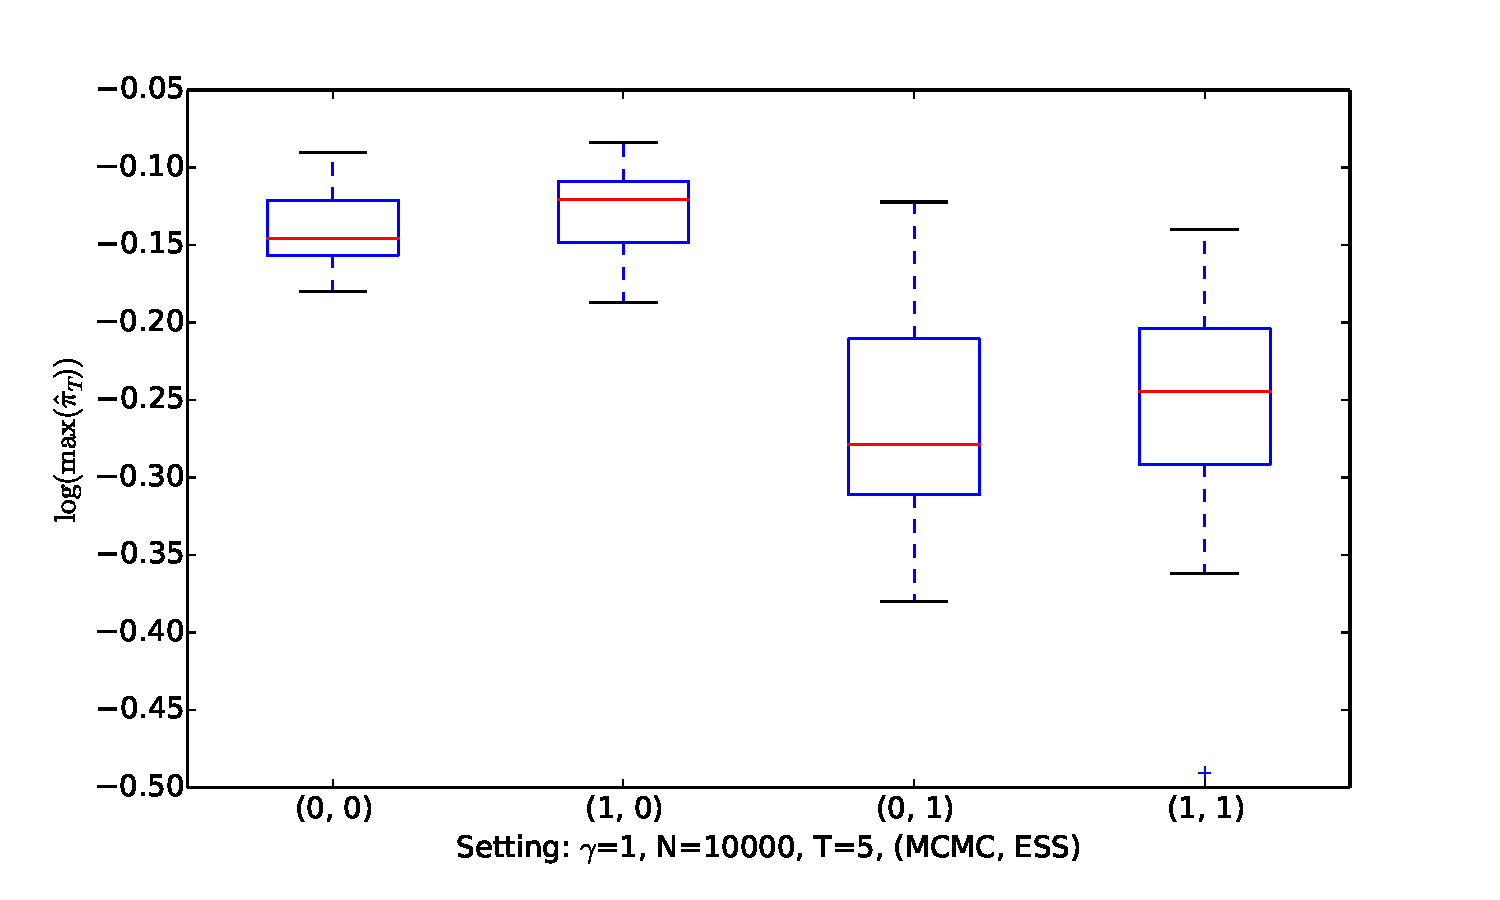
\includegraphics[width=\textwidth]{loglik_mcmc_ess/T5_gamma1_N10000.pdf}
        %\includegraphics[width=0.3\linewidth, height=0.15\textheight]{prob1_6_2}
        %\caption{$dt=0.1$}
        %\label{fig:prob1_6_2}
    \end{minipage}%
    \begin{minipage}{0.5\textwidth}
        \centering
        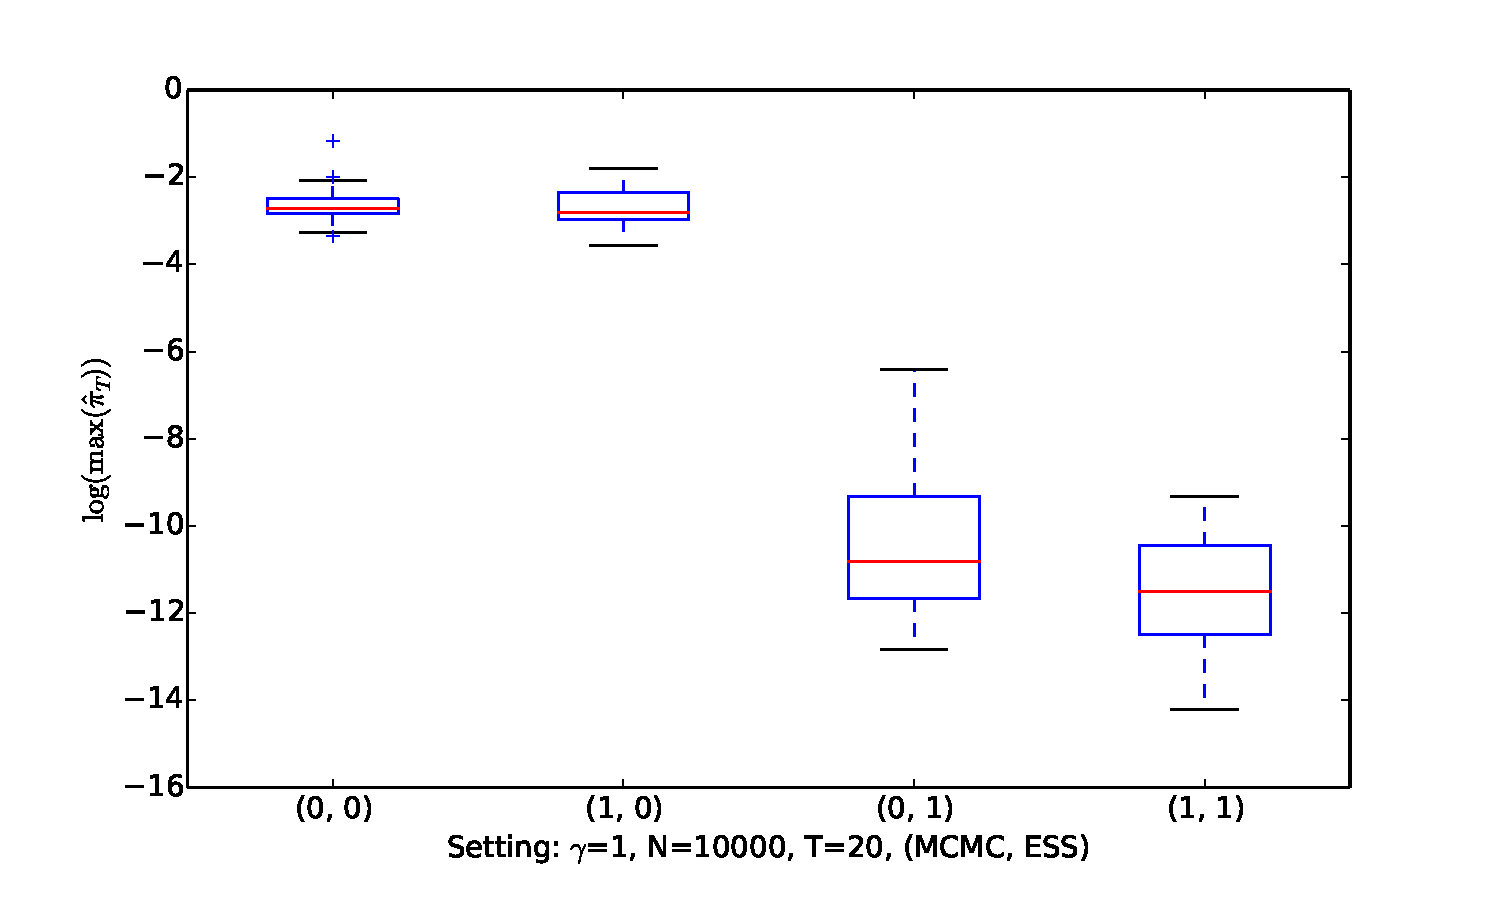
\includegraphics[width=\textwidth]{loglik_mcmc_ess/T20_gamma1_N10000.pdf}
    \end{minipage}
    \begin{minipage}{0.5\textwidth}
        \centering
        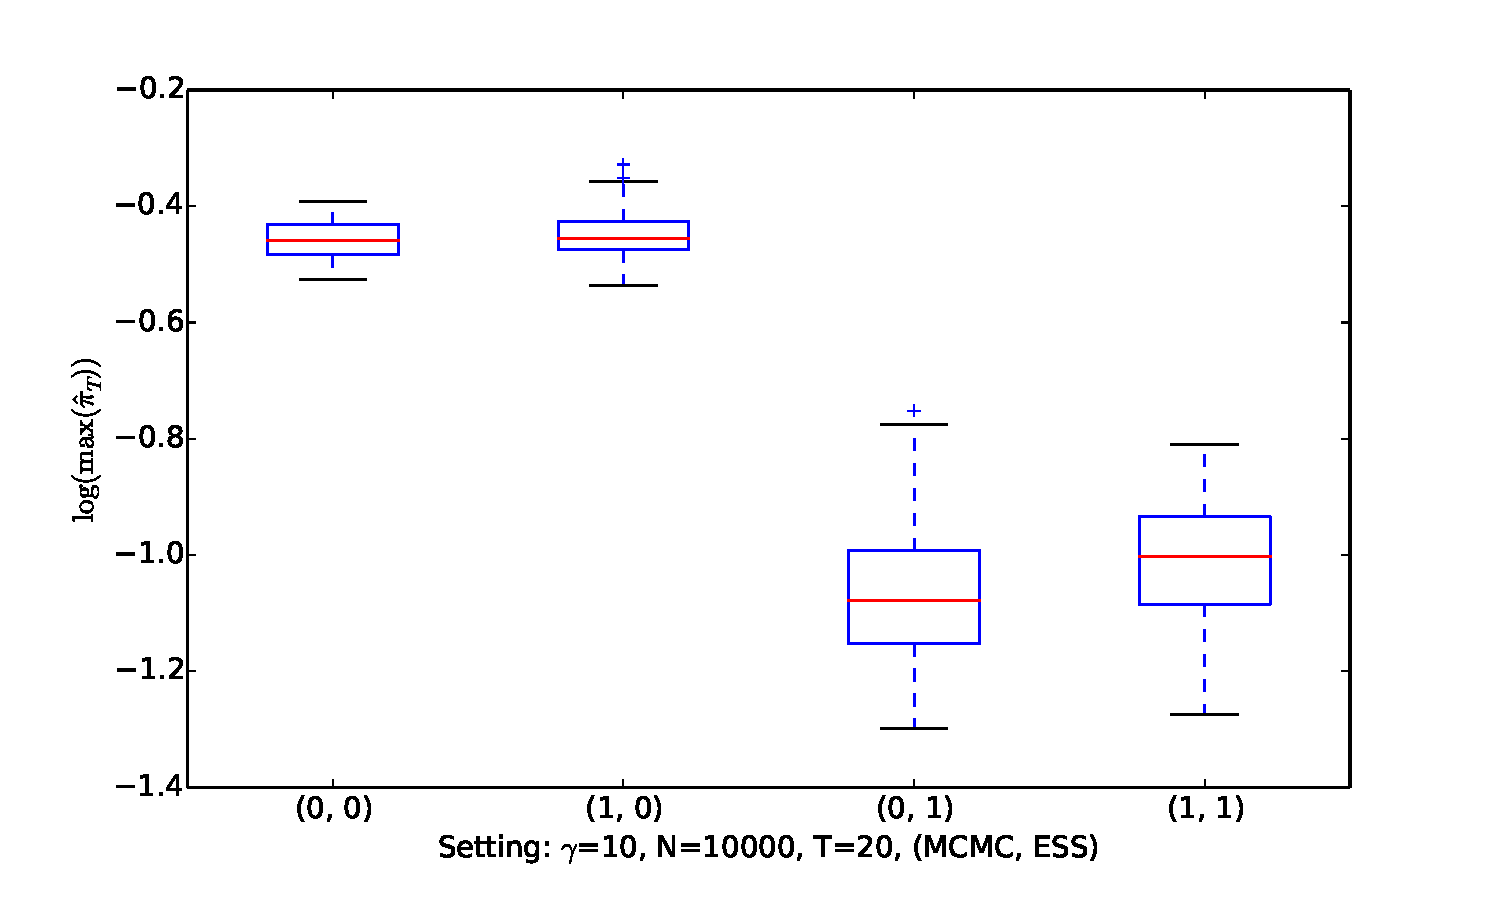
\includegraphics[width=\textwidth]{loglik_mcmc_ess/T20_gamma10_N10000.pdf}
    \end{minipage}%
    \begin{minipage}{0.5\textwidth}
        \centering
        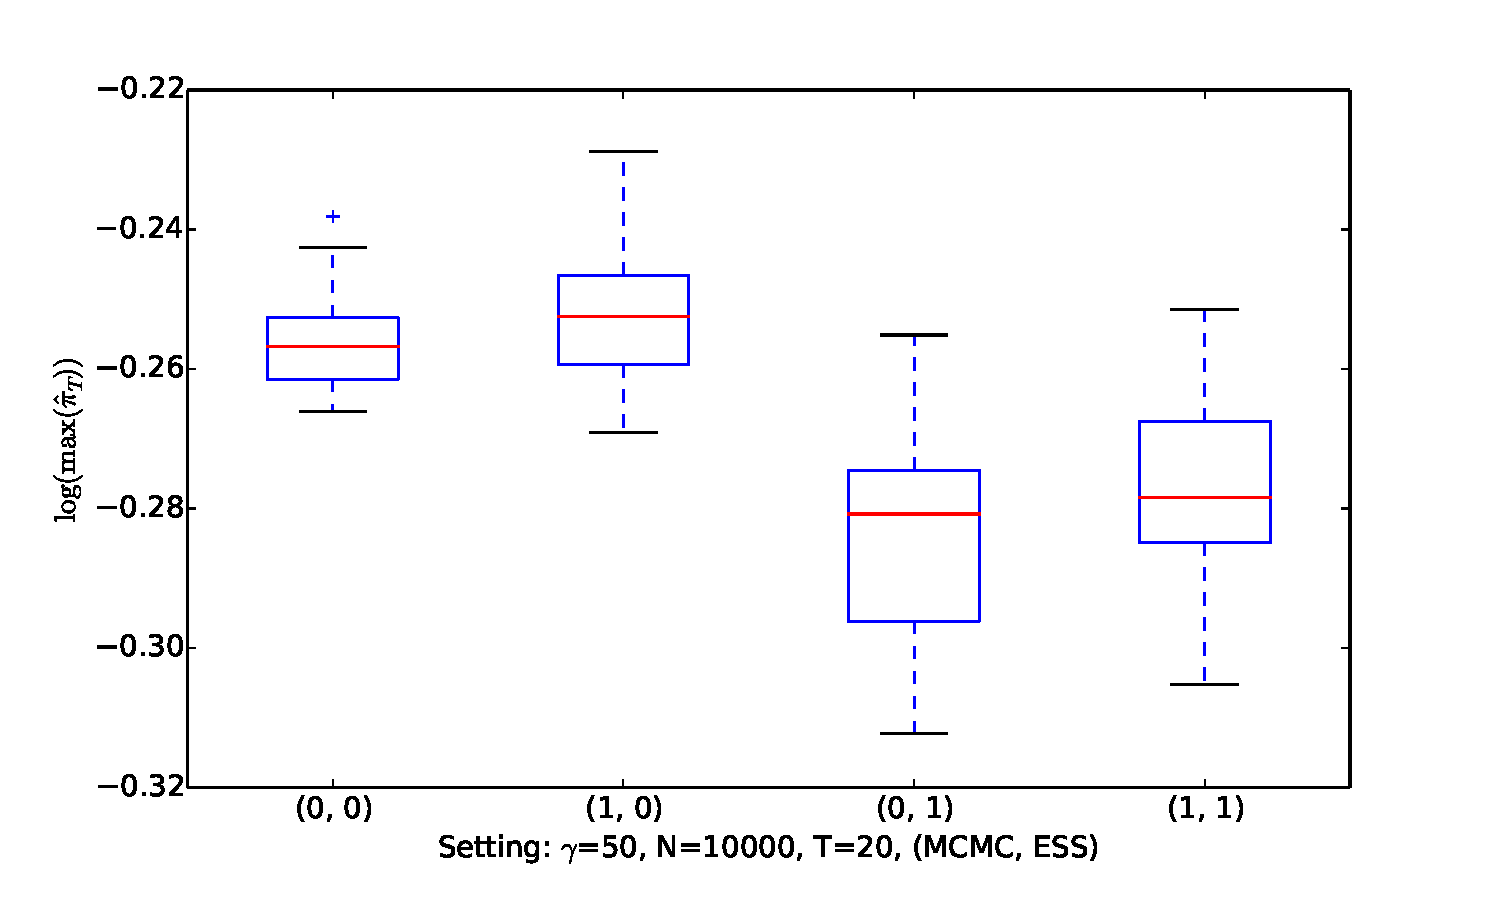
\includegraphics[width=\textwidth]{loglik_mcmc_ess/T20_gamma50_N10000.pdf}
    \end{minipage}
    \begin{minipage}{0.5\textwidth}
        \centering
        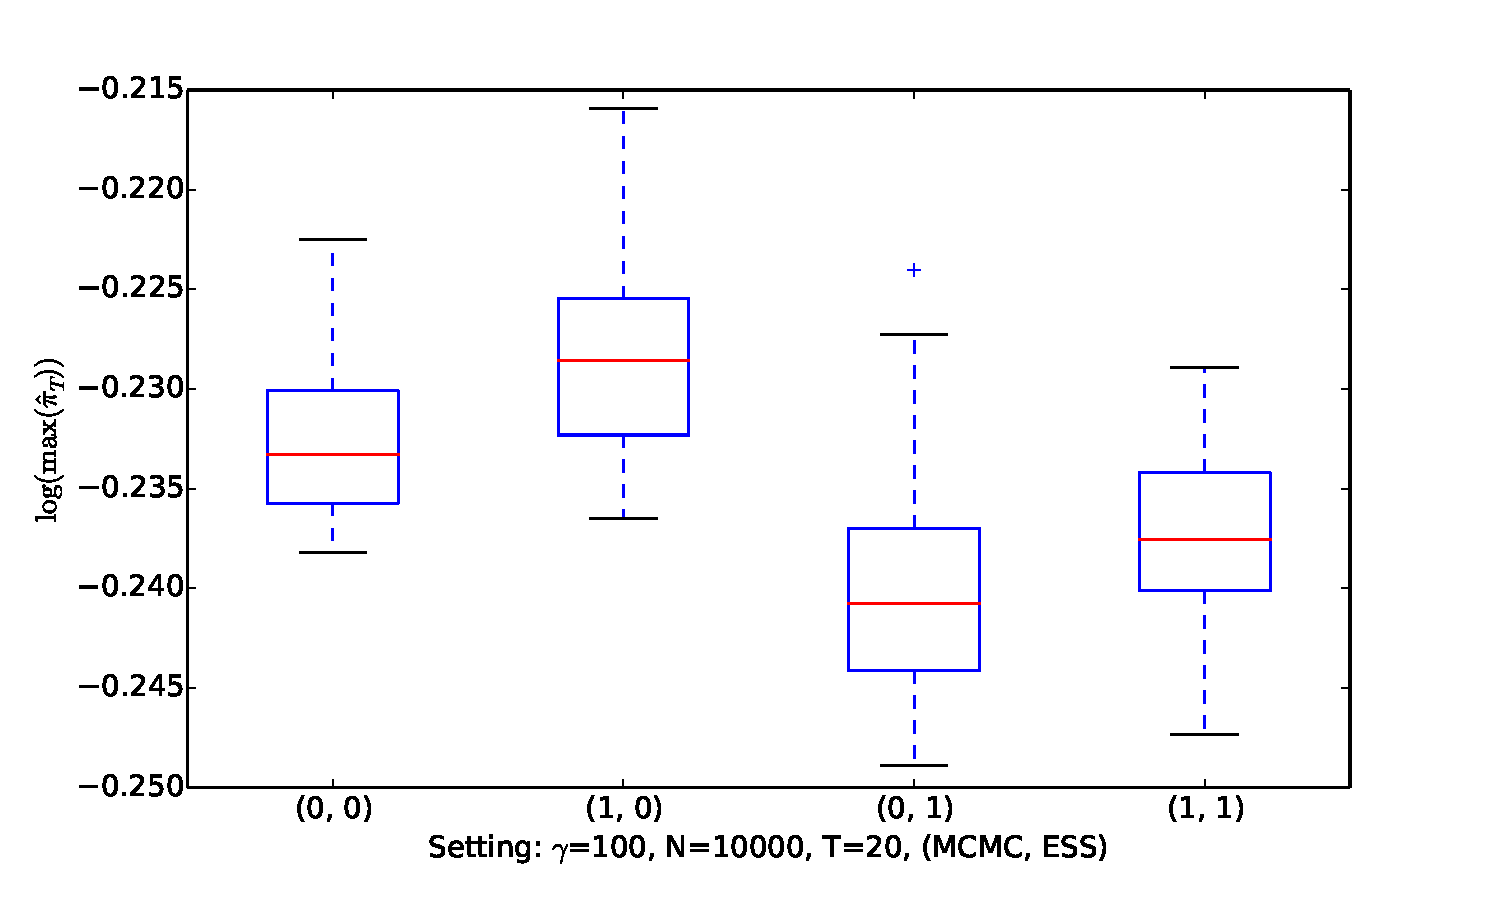
\includegraphics[width=\textwidth]{loglik_mcmc_ess/T20_gamma100_N10000.pdf}
    \end{minipage}%
    \begin{minipage}{0.5\textwidth}
        \centering
        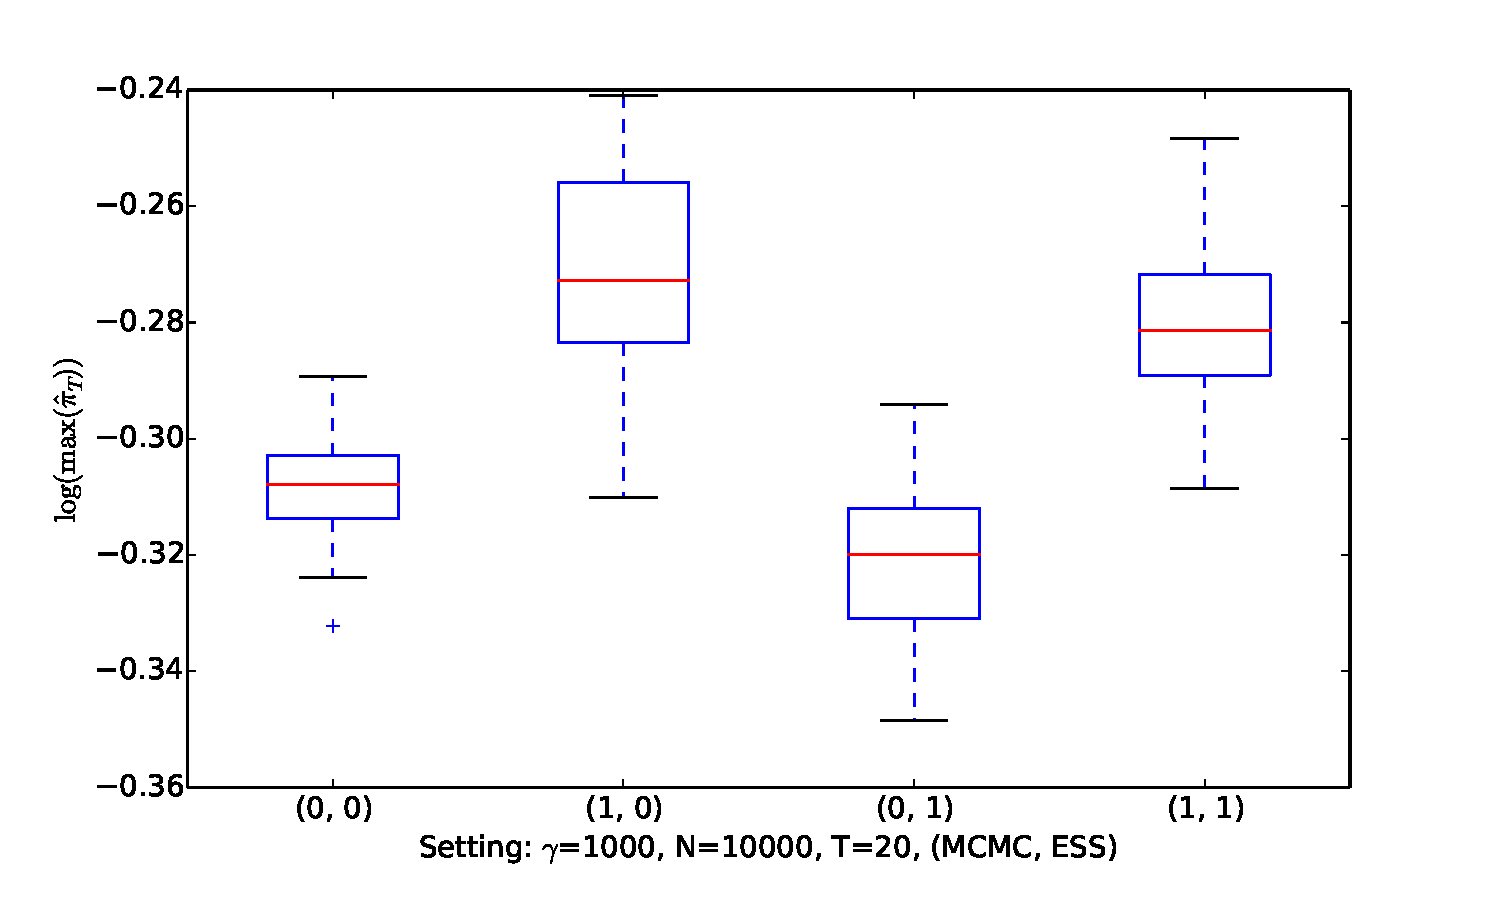
\includegraphics[width=\textwidth]{loglik_mcmc_ess/T20_gamma1000_N10000.pdf}
    \end{minipage}
    \begin{minipage}{0.5\textwidth}
        \centering
        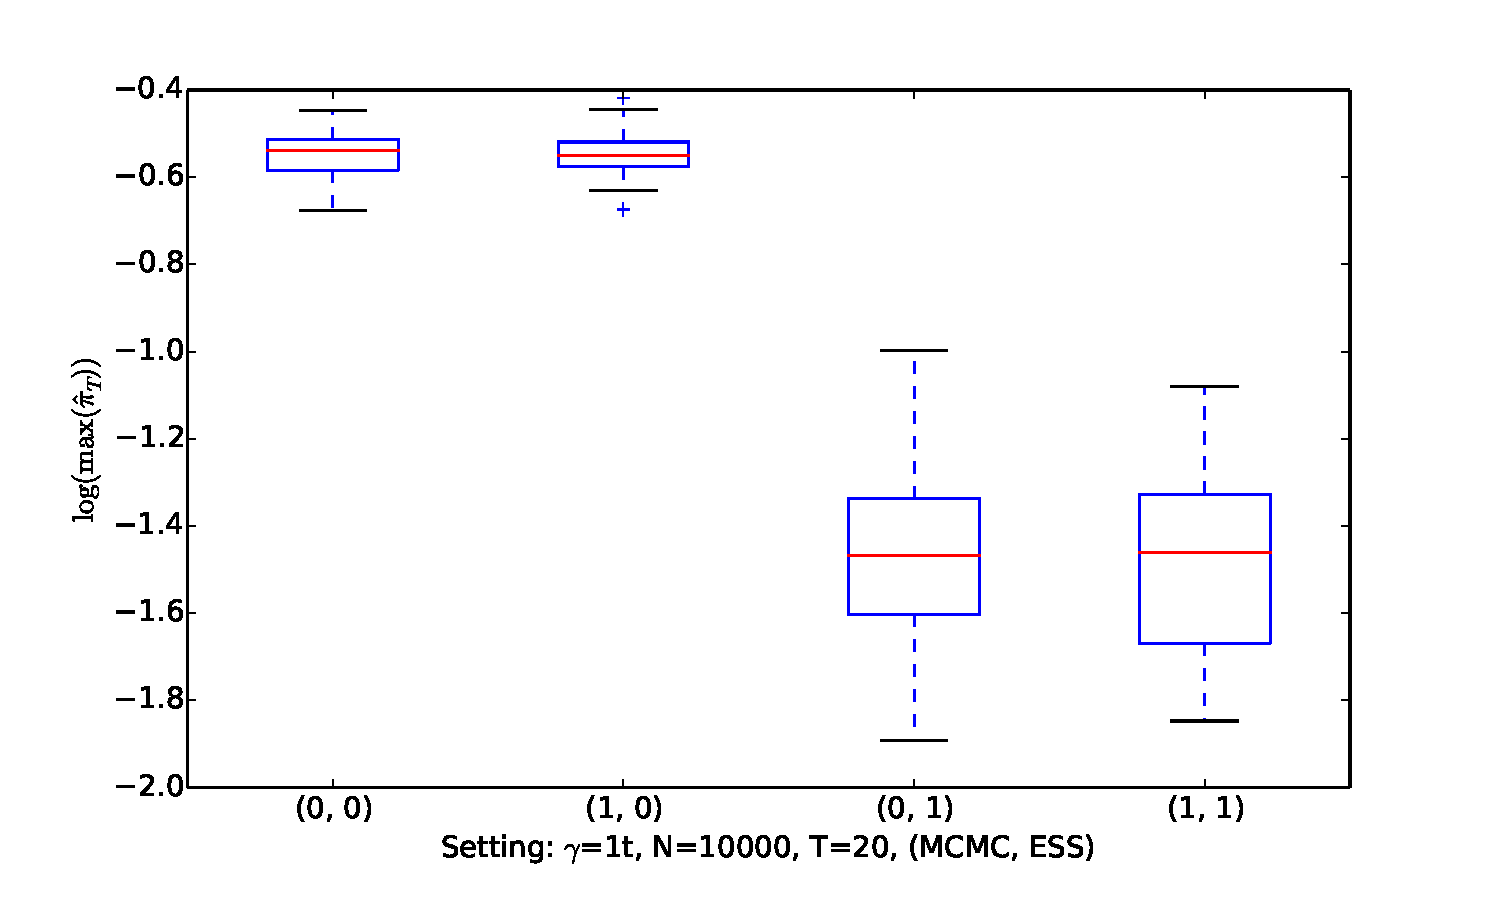
\includegraphics[width=\textwidth]{loglik_mcmc_ess/T20_gamma1t_N10000.pdf}
    \end{minipage}%
    \begin{minipage}{0.5\textwidth}
        \centering
        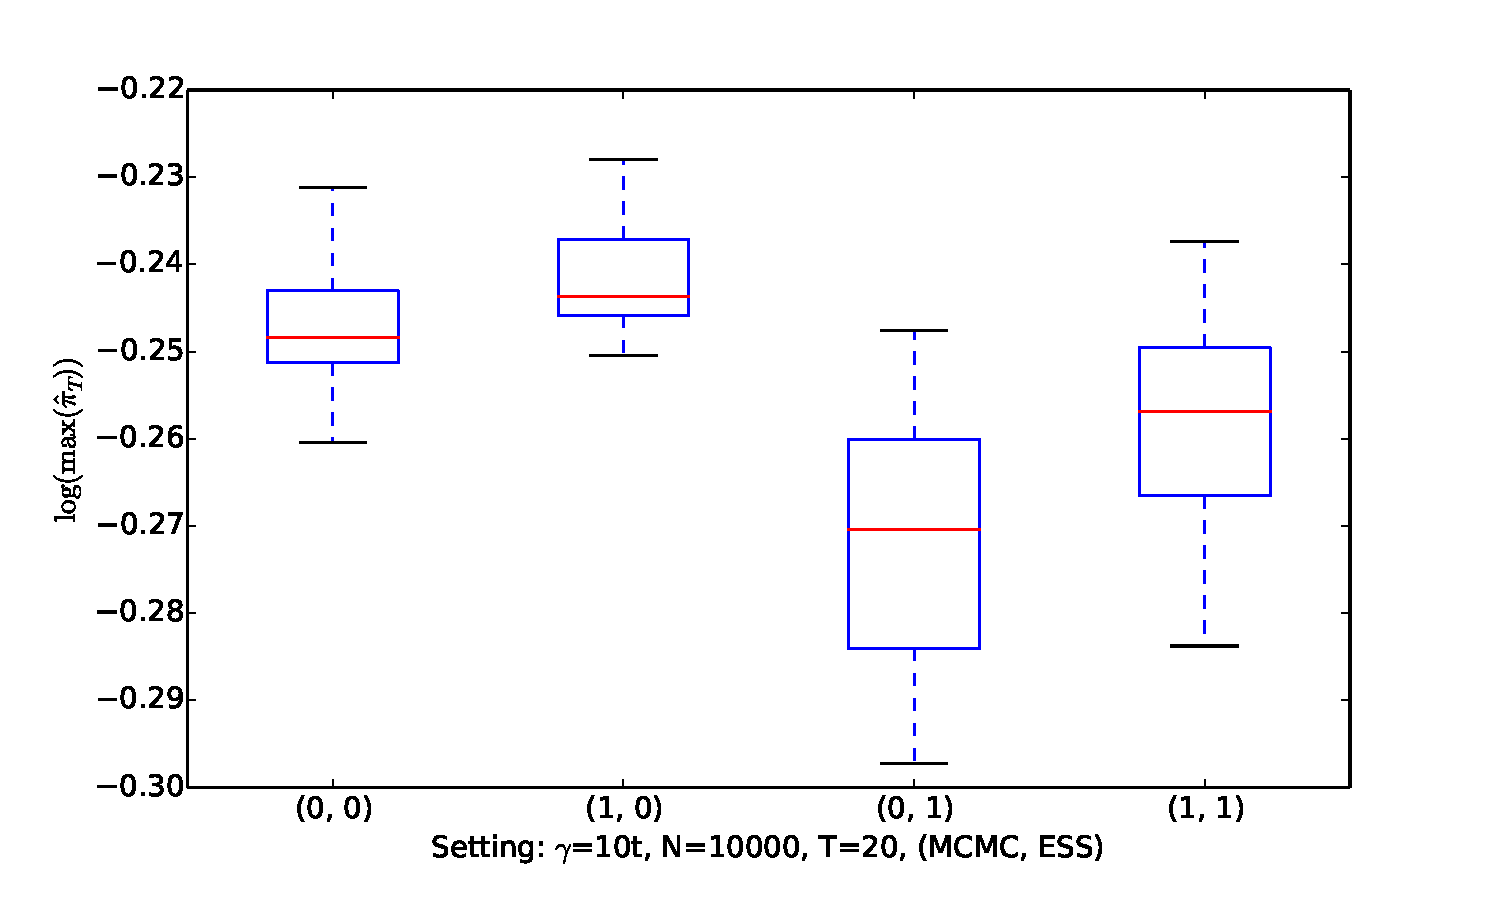
\includegraphics[width=\textwidth]{loglik_mcmc_ess/T20_gamma10t_N10000.pdf}
    \end{minipage}
    \begin{minipage}{0.5\textwidth}
        \centering
        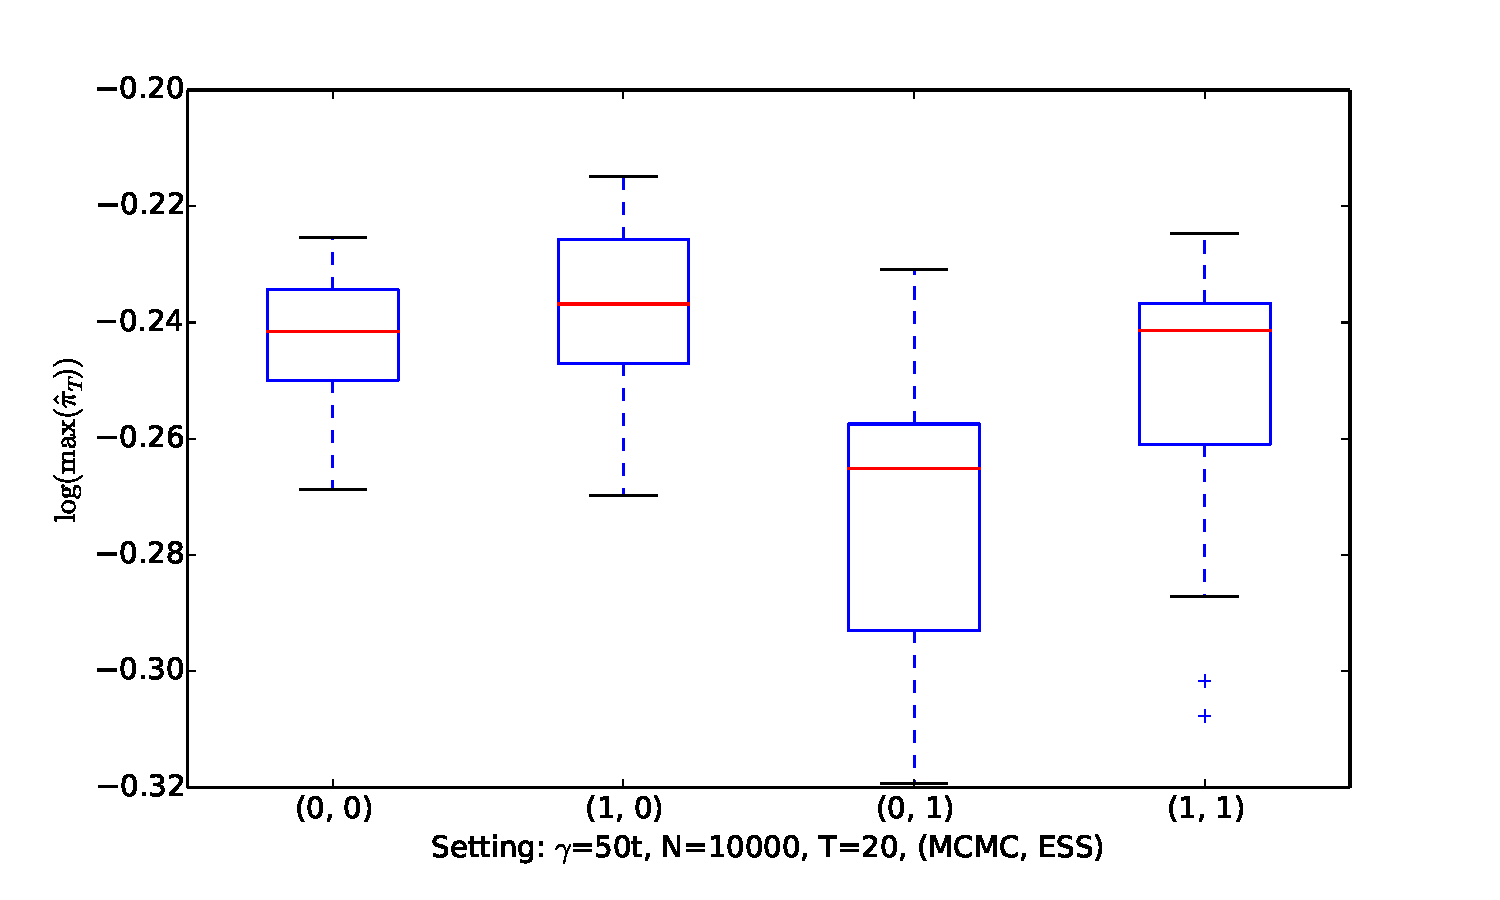
\includegraphics[width=\textwidth]{loglik_mcmc_ess/T20_gamma50t_N10000.pdf}
    \end{minipage}%
    \begin{minipage}{0.5\textwidth}
        \centering
        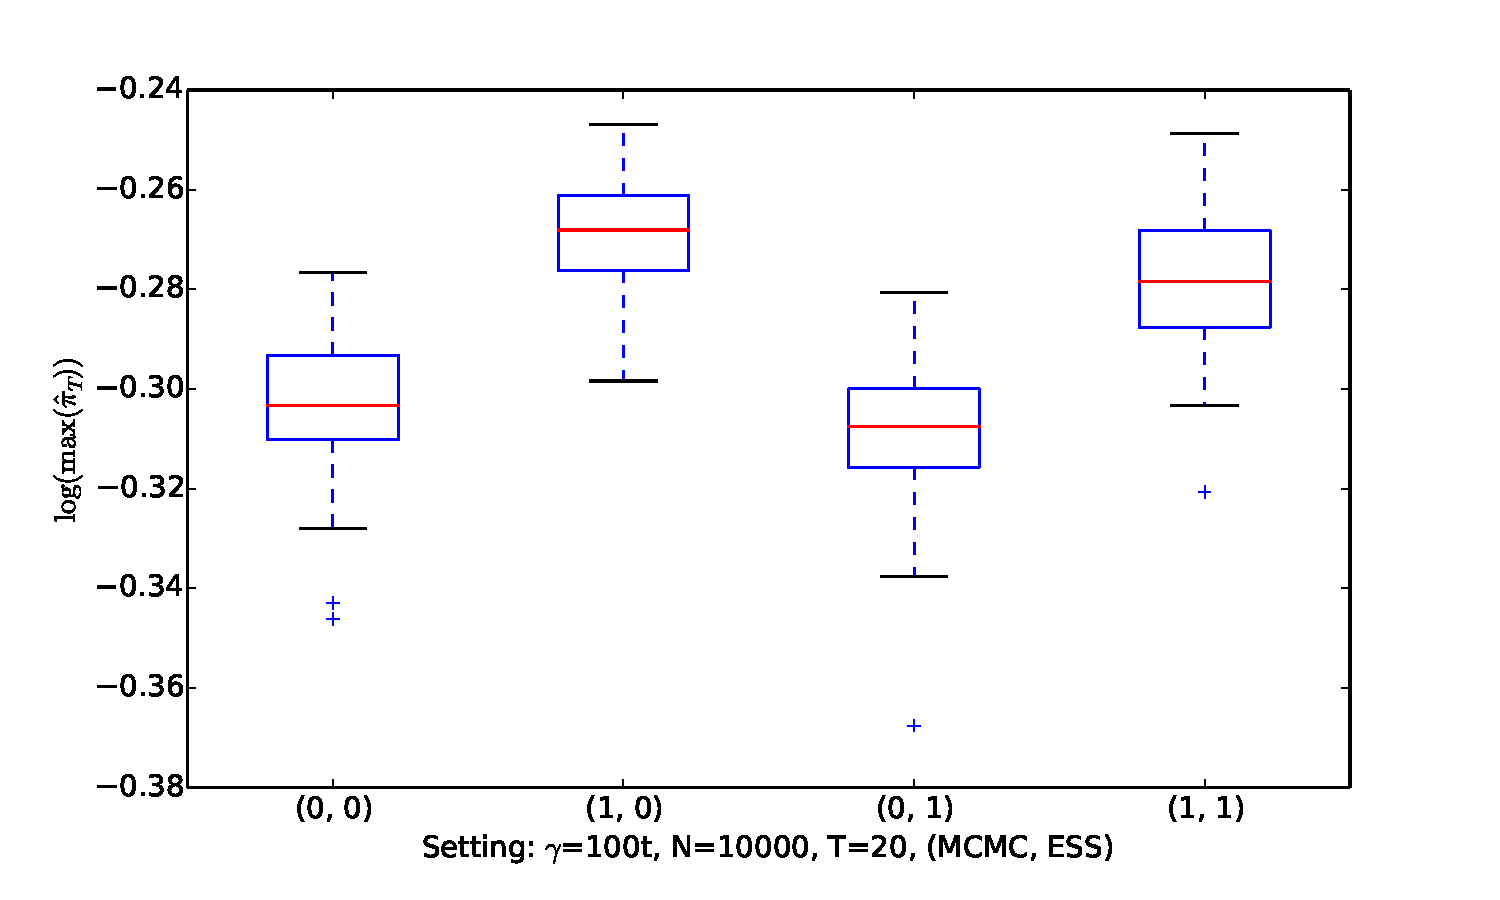
\includegraphics[width=\textwidth]{loglik_mcmc_ess/T20_gamma100t_N10000.pdf}
    \end{minipage}
    \caption{The $\log\pi_T(\hat{u}^*_{0:t})$ box-plots of 30 independent runs ($T=20$ and $N=10000$) of the algorithms.}
    \label{fig:ess}
\end{figure}

\begin{figure}[!htbp]
    \centering
    \begin{minipage}{.5\textwidth}
        \centering
        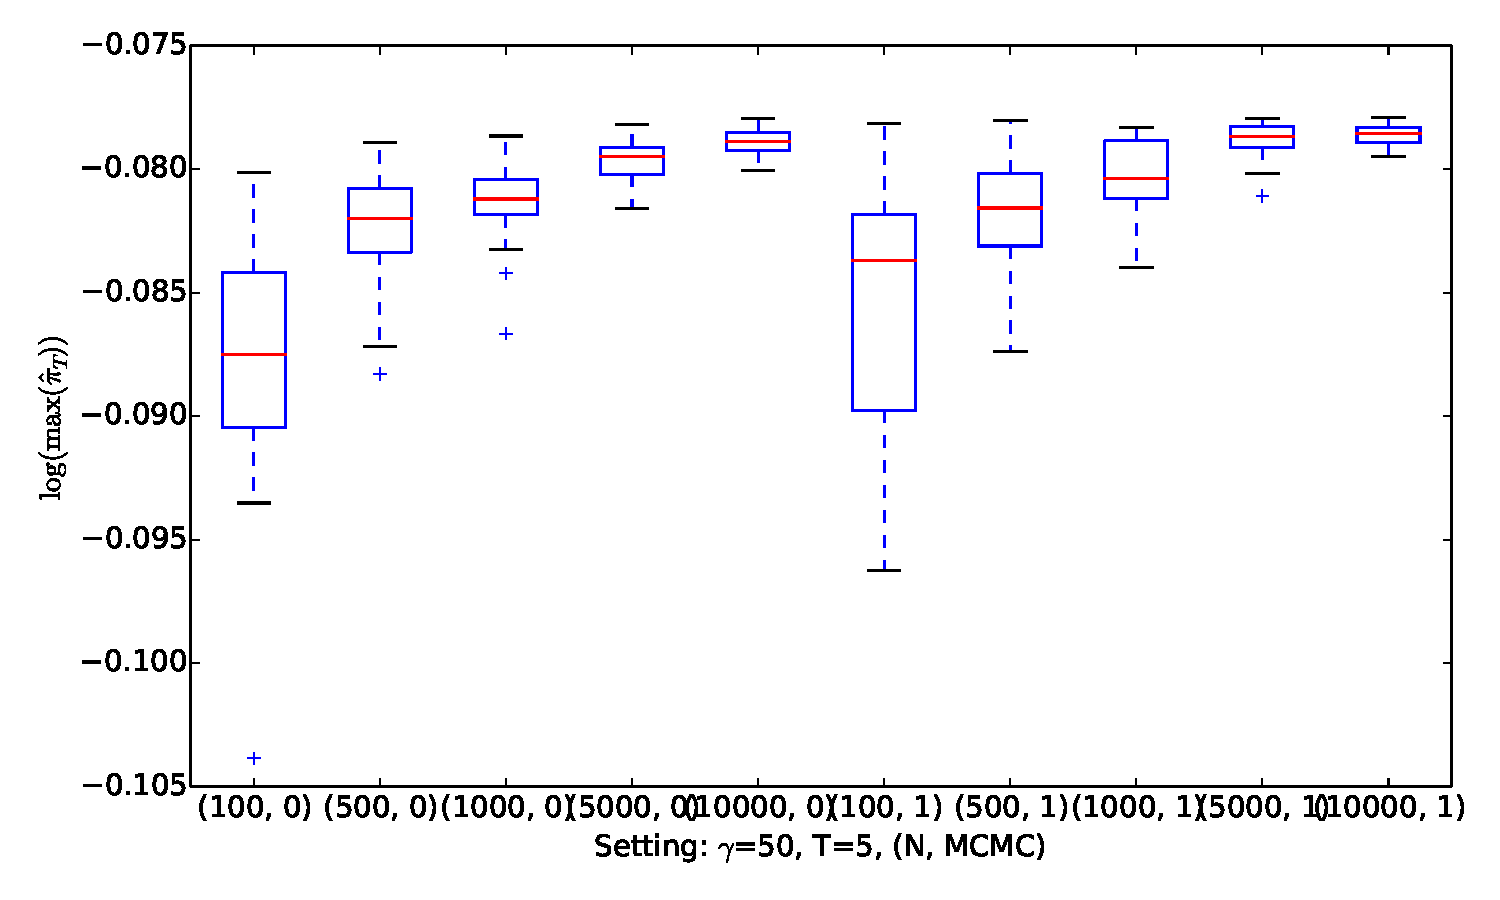
\includegraphics[width=\textwidth]{loglik_t_gs_n/T5_gamma50.pdf}
    \end{minipage}%
    \begin{minipage}{0.5\textwidth}
        \centering
        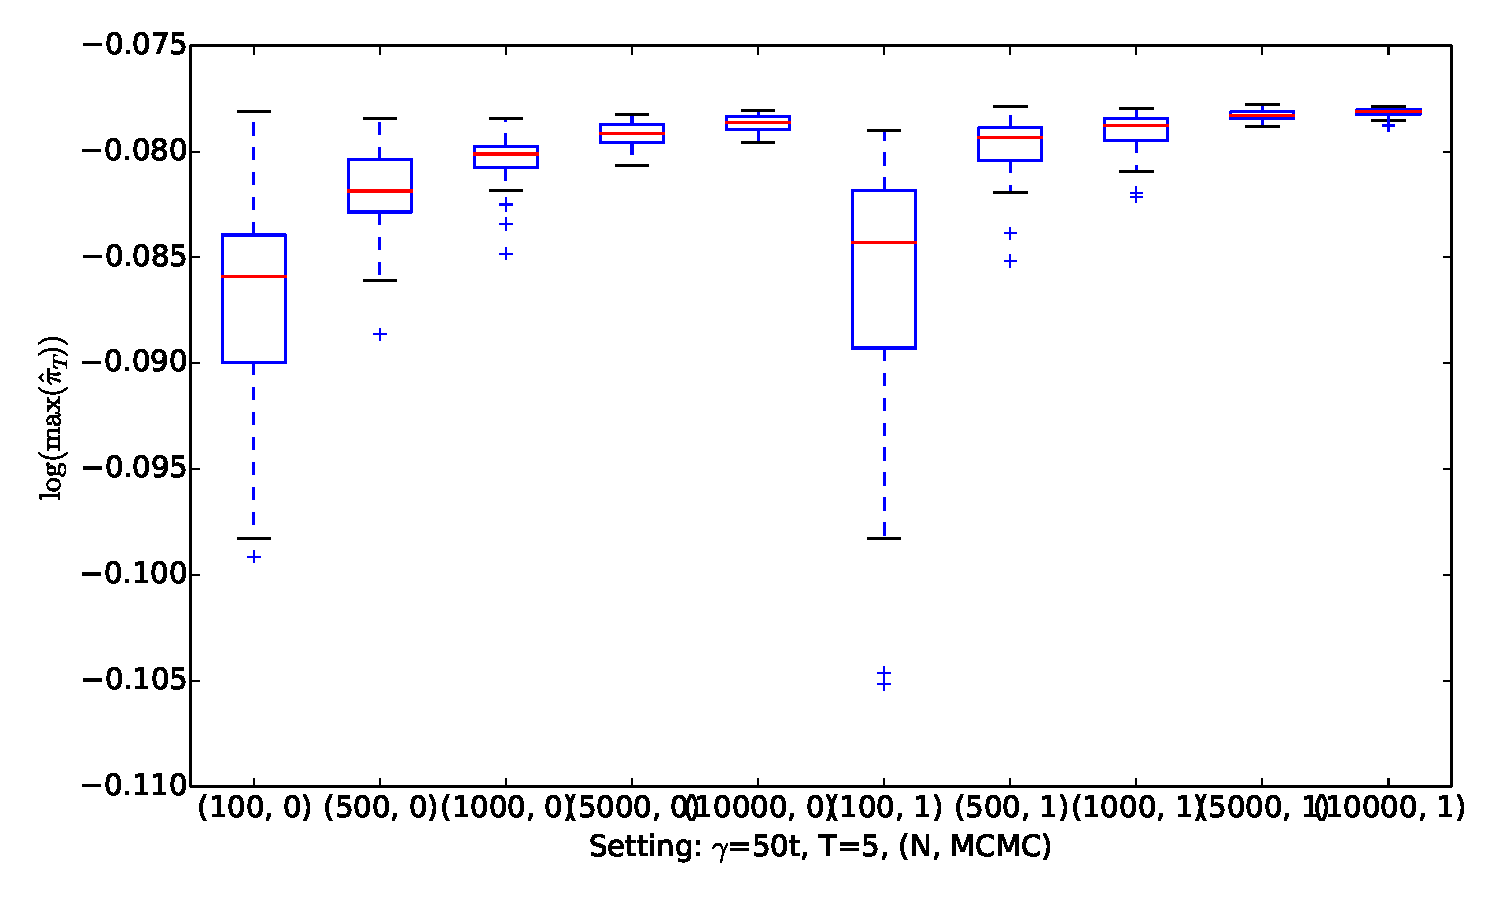
\includegraphics[width=\textwidth]{loglik_t_gs_n/T5_gamma50t.pdf}
    \end{minipage}
    \begin{minipage}{0.5\textwidth}
        \centering
        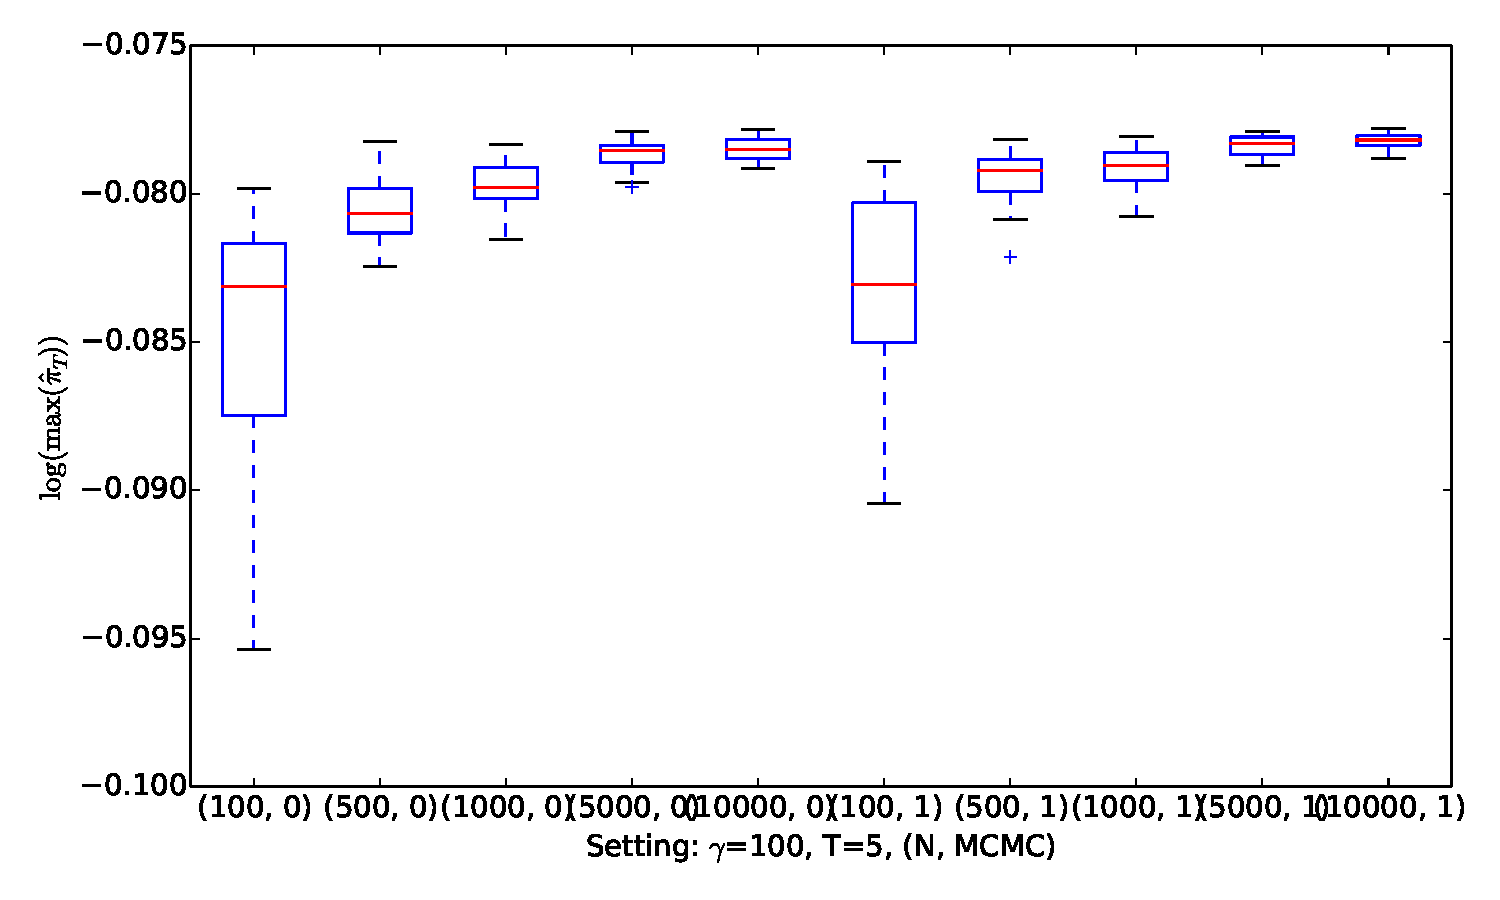
\includegraphics[width=\textwidth]{loglik_t_gs_n/T5_gamma100.pdf}
    \end{minipage}%
    \begin{minipage}{0.5\textwidth}
        \centering
        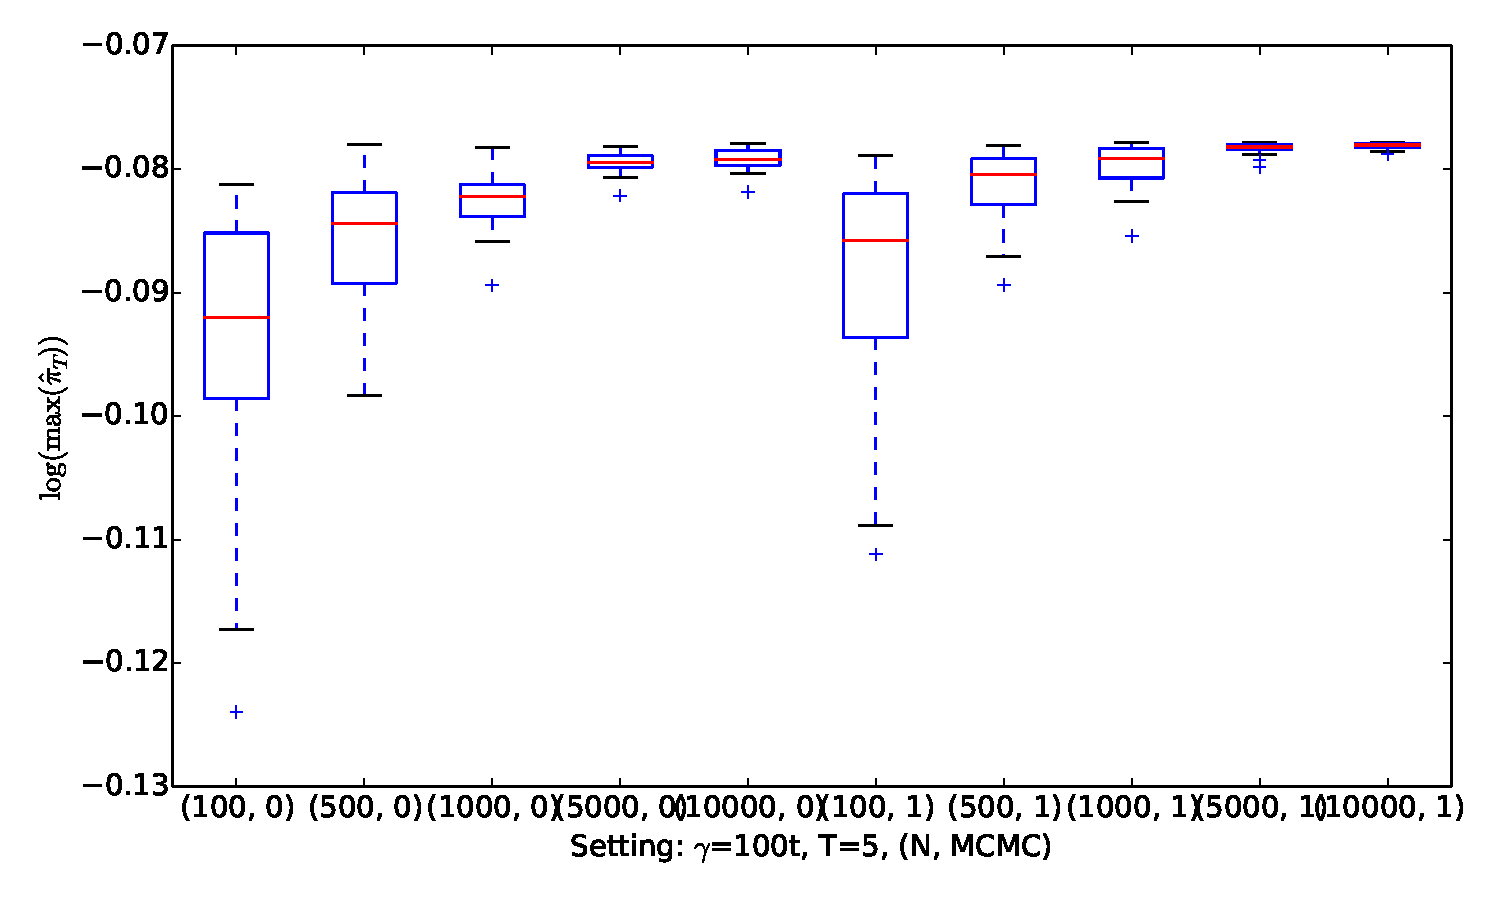
\includegraphics[width=\textwidth]{loglik_t_gs_n/T5_gamma100t.pdf}
    \end{minipage}
    \begin{minipage}{0.5\textwidth}
        \centering
        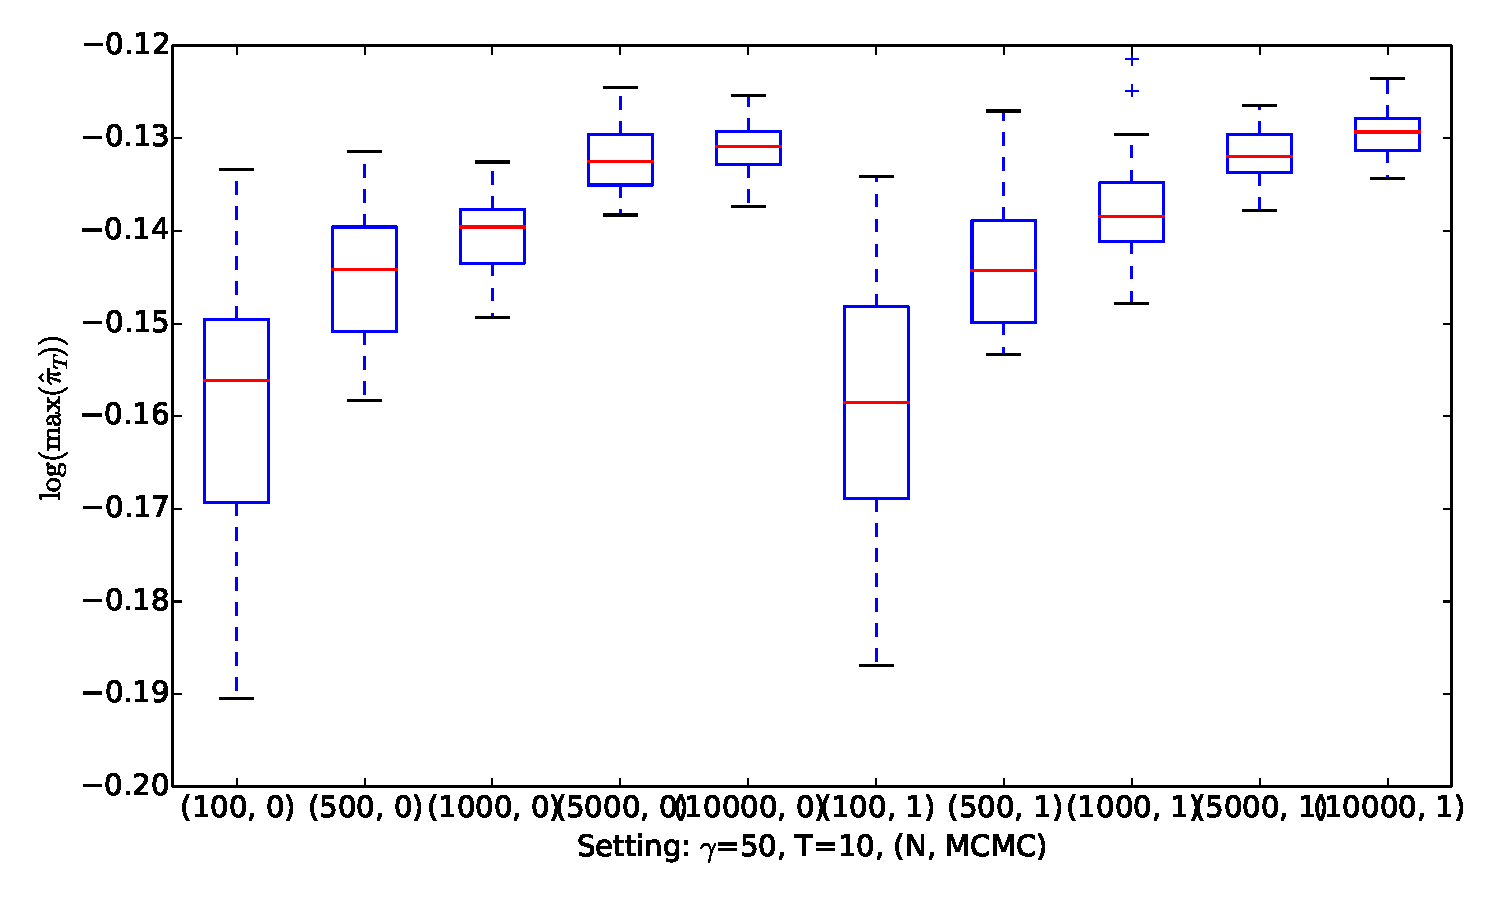
\includegraphics[width=\textwidth]{loglik_t_gs_n/T10_gamma50.pdf}
    \end{minipage}%
    \begin{minipage}{0.5\textwidth}
        \centering
        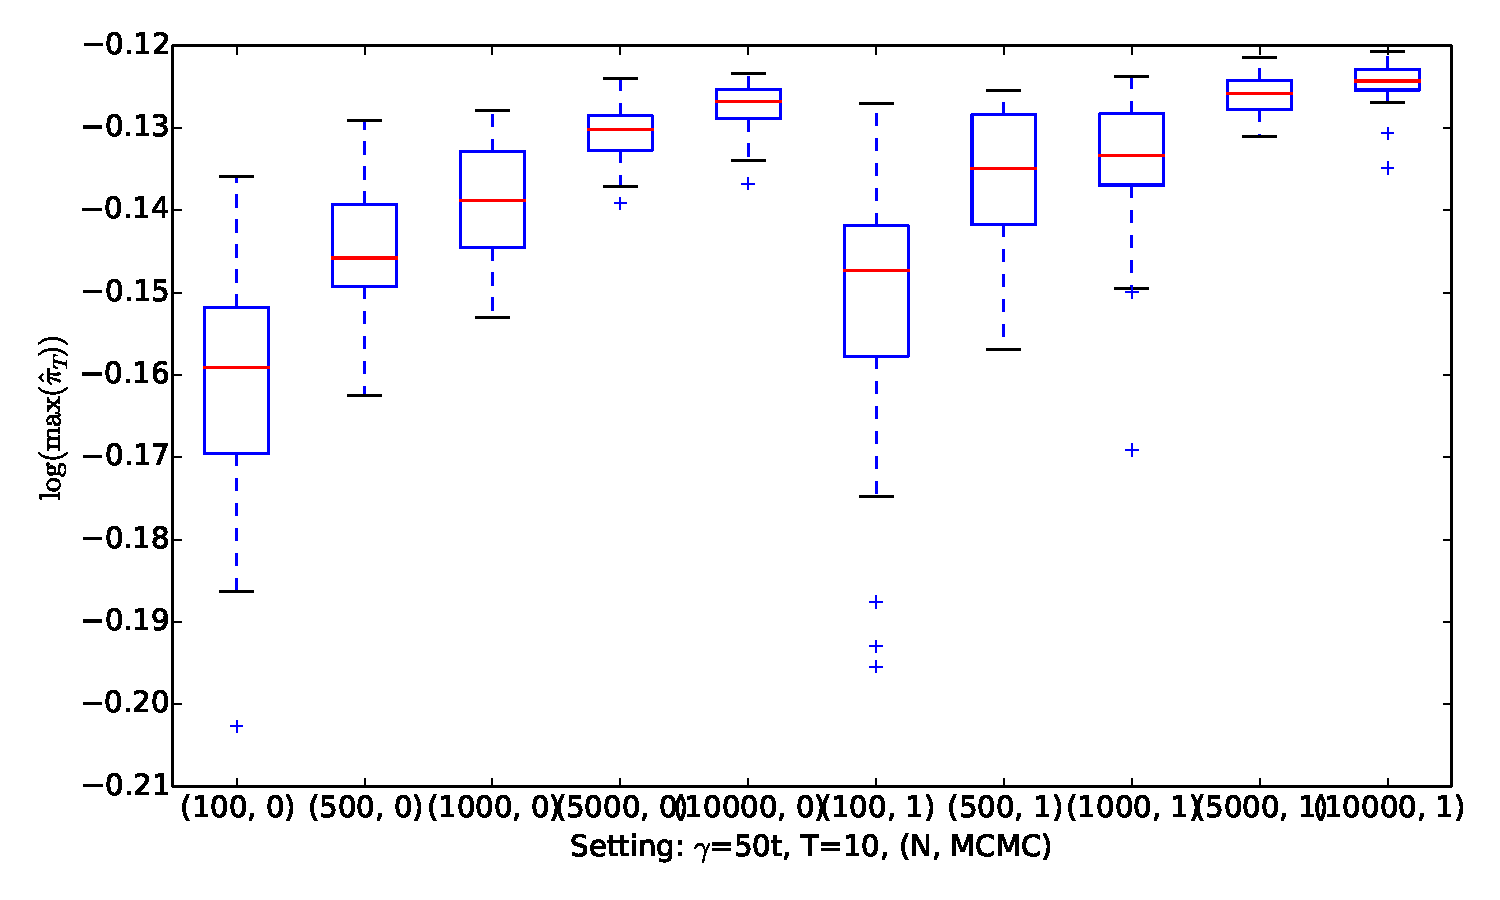
\includegraphics[width=\textwidth]{loglik_t_gs_n/T10_gamma50t.pdf}
    \end{minipage}
    \begin{minipage}{0.5\textwidth}
        \centering
        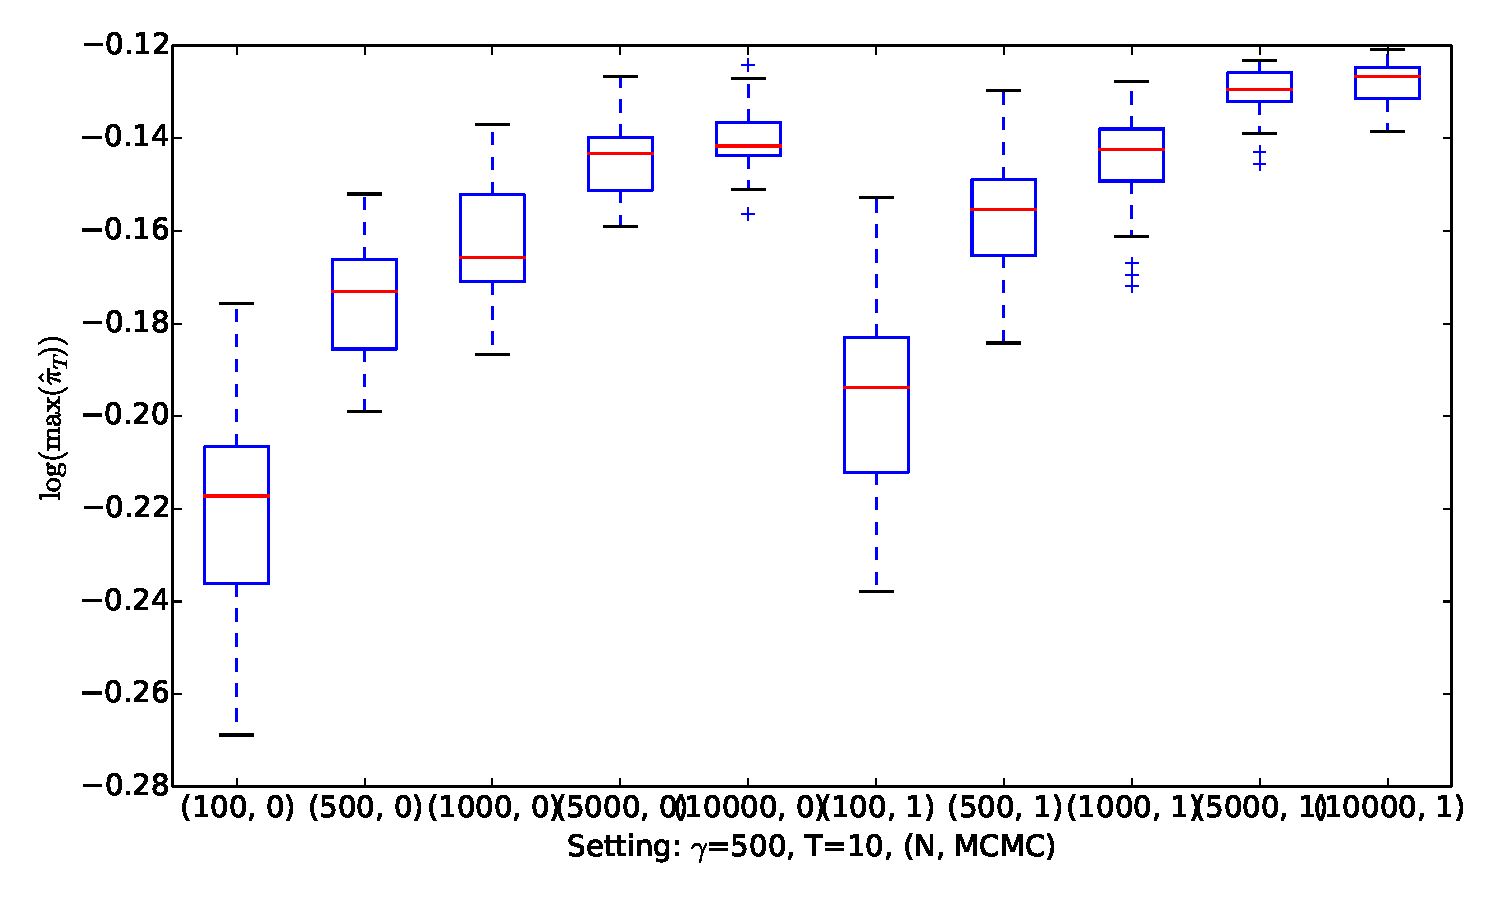
\includegraphics[width=\textwidth]{loglik_t_gs_n/T10_gamma500.pdf}
    \end{minipage}%
    \begin{minipage}{0.5\textwidth}
        \centering
        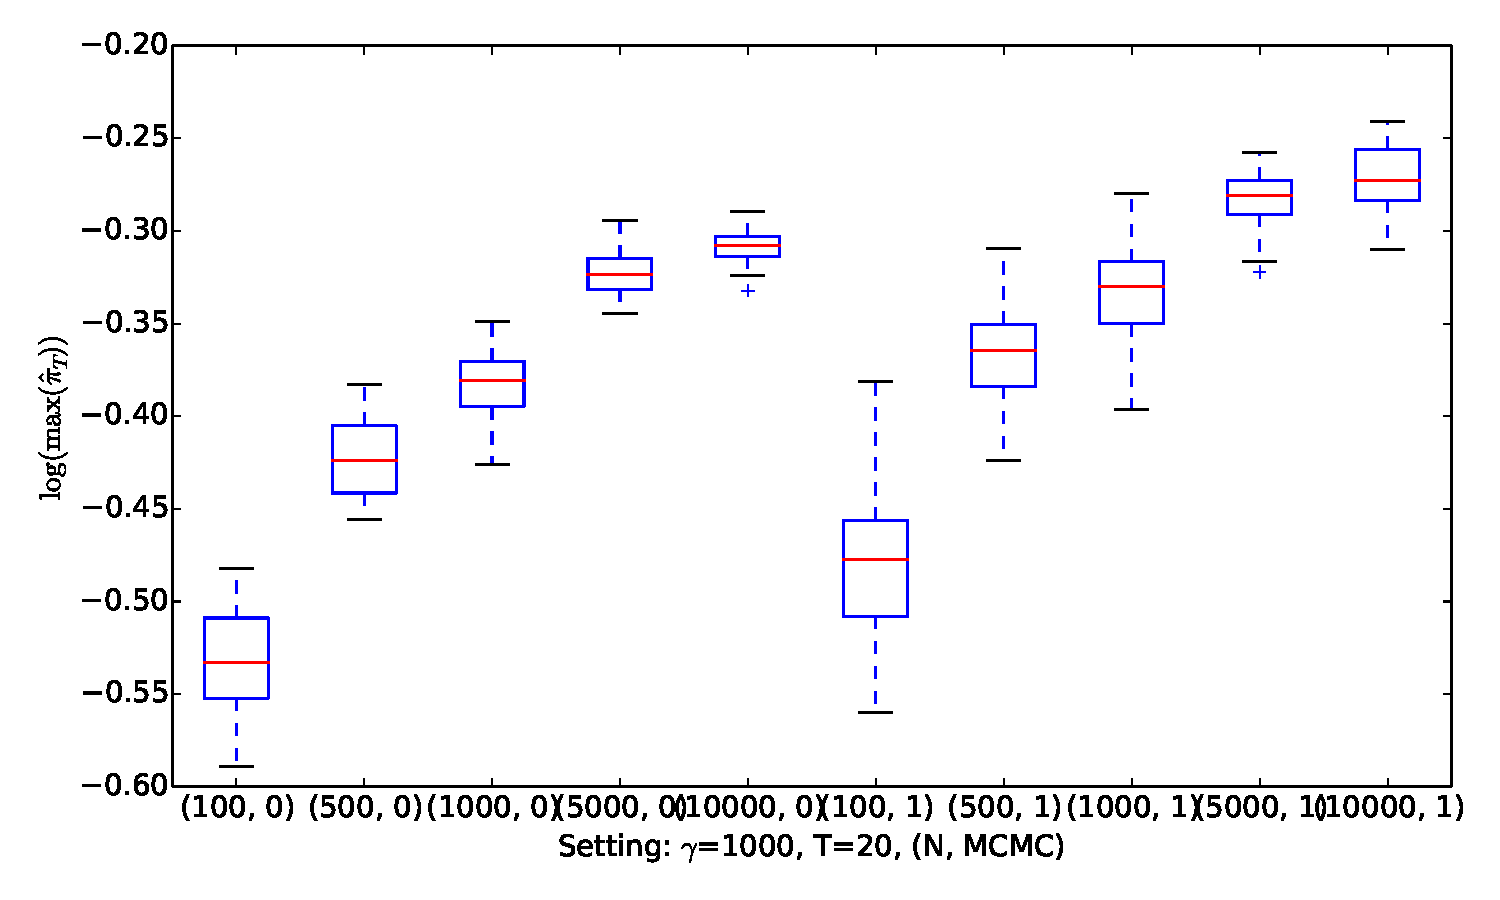
\includegraphics[width=\textwidth]{loglik_t_gs_n/T20_gamma1000.pdf}
    \end{minipage}
    \begin{minipage}{0.5\textwidth}
        \centering
        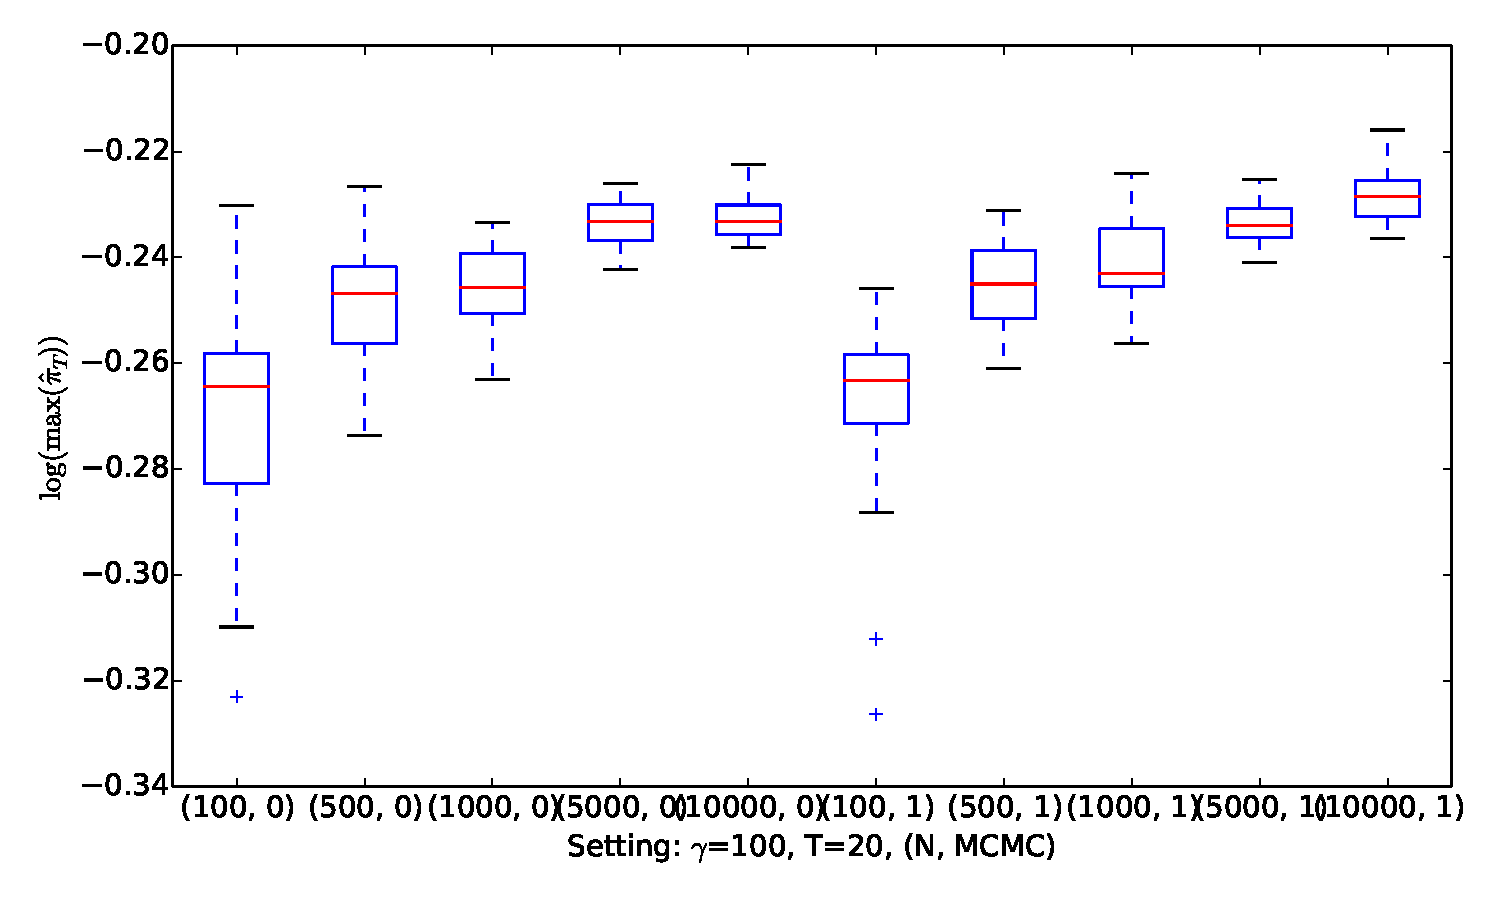
\includegraphics[width=\textwidth]{loglik_t_gs_n/T20_gamma100.pdf}
    \end{minipage}%
    \begin{minipage}{0.5\textwidth}
        \centering
        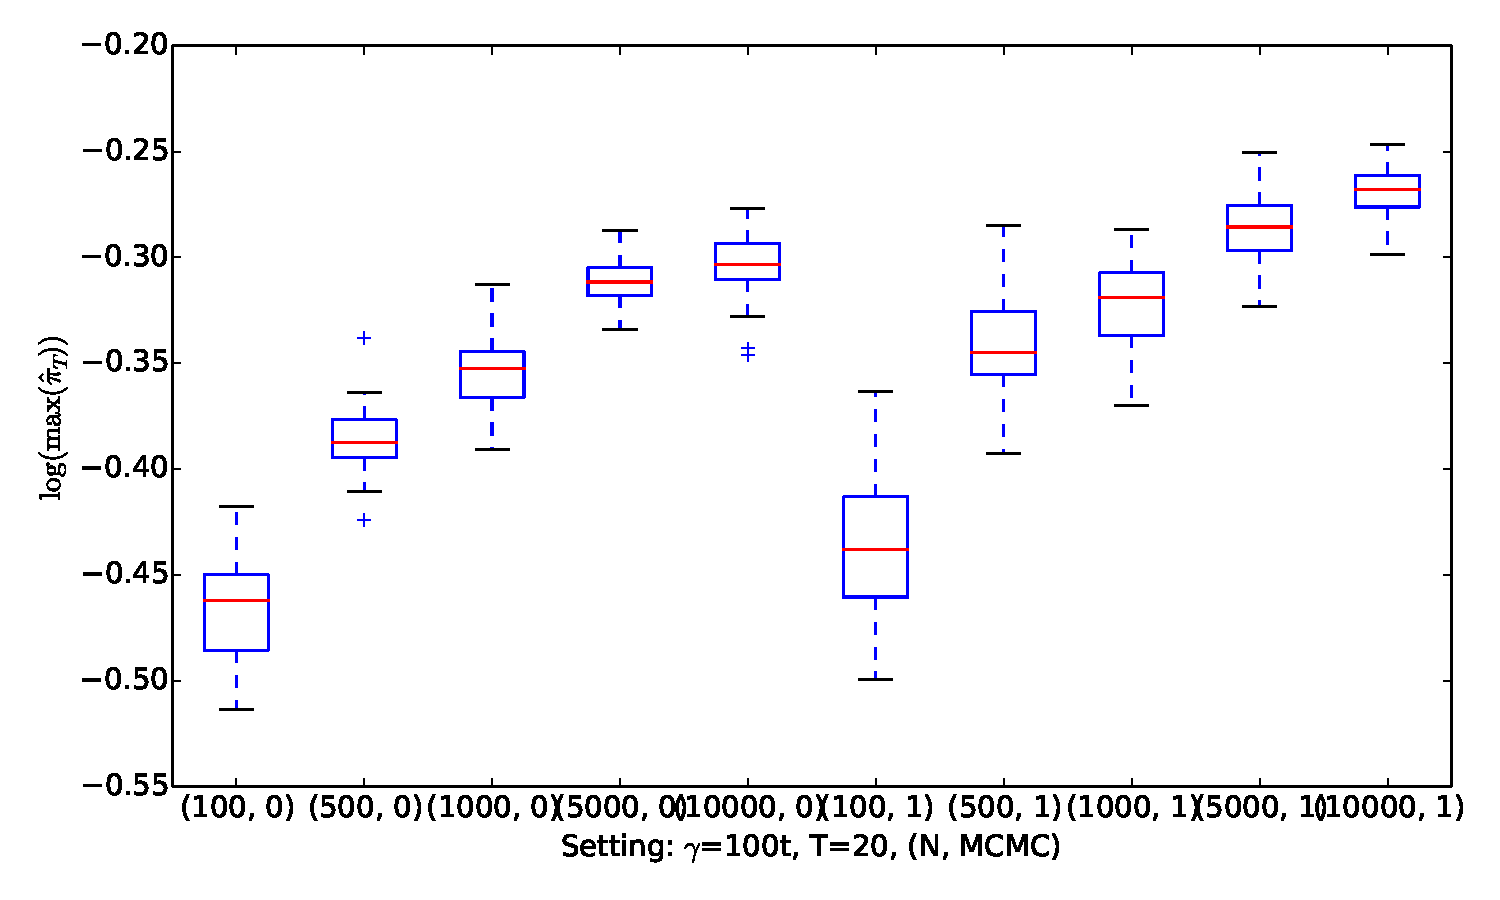
\includegraphics[width=\textwidth]{loglik_t_gs_n/T20_gamma100t.pdf}
    \end{minipage}
    \caption{The $\log\pi_T(\hat{u}^*_{0:t})$ box-plots of 30 independent runs with various settings. The leftmost/rightmost $5$ box-plots in each figure are for the runs without/with resample-move step.}
    \label{fig:rm}
\end{figure}

\begin{figure}[!htbp]
    \centering
    \begin{minipage}{.5\textwidth}
        \centering
        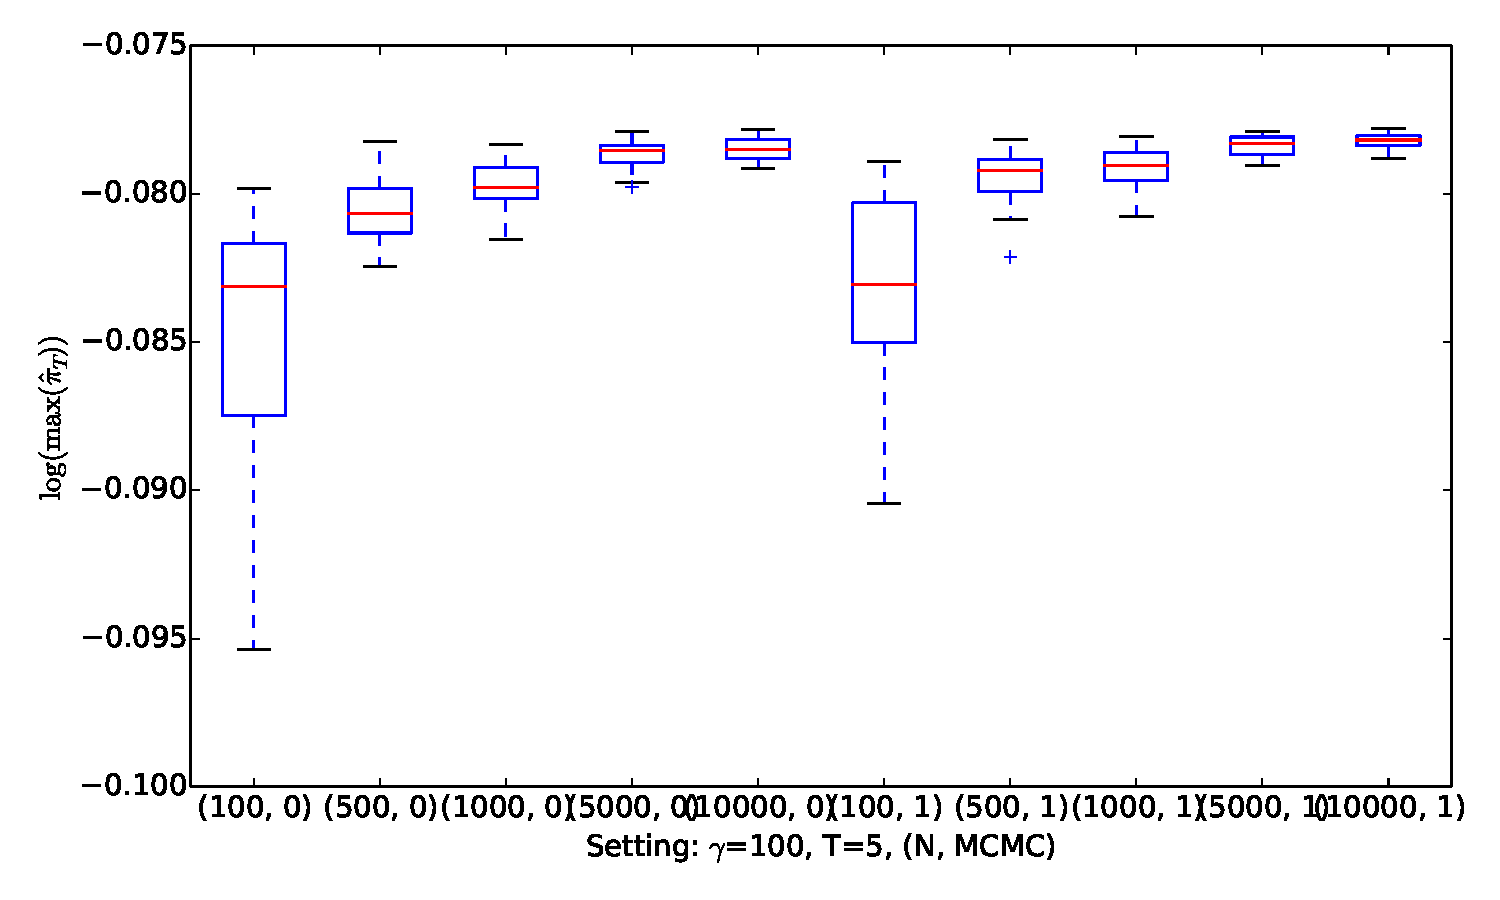
\includegraphics[width=\textwidth]{loglik_t_gs_n/T5_gamma100.pdf}
        %\includegraphics[width=0.3\linewidth, height=0.15\textheight]{prob1_6_2}
        %\caption{$dt=0.1$}
        %\label{fig:prob1_6_2}
    \end{minipage}%
    \begin{minipage}{0.5\textwidth}
        \centering
        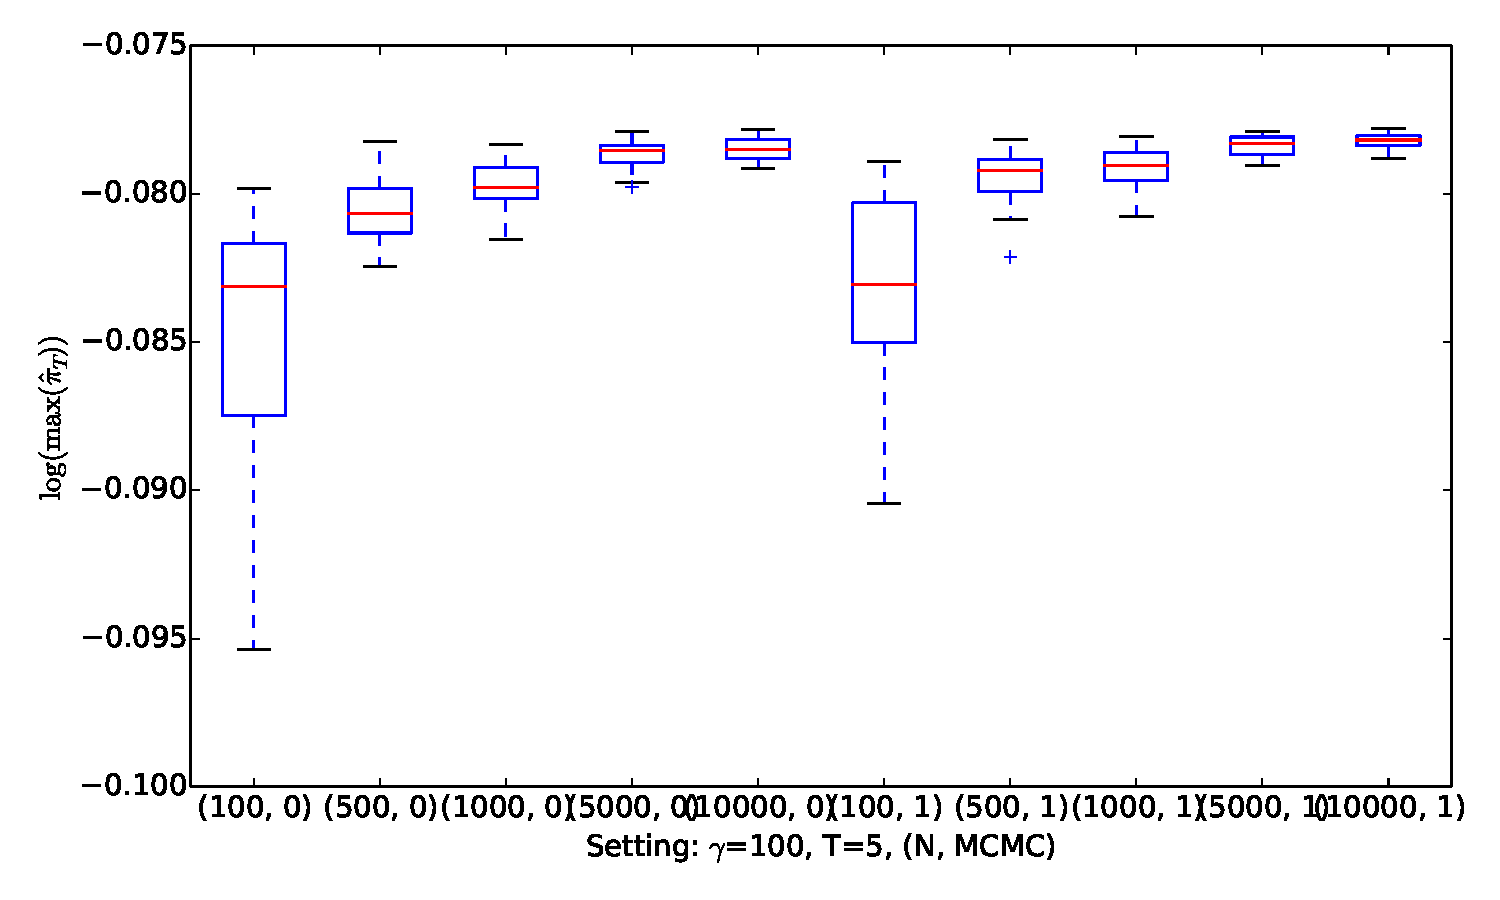
\includegraphics[width=\textwidth]{loglik_t_gs_n/T5_gamma100.pdf}
    \end{minipage}
    \begin{minipage}{0.5\textwidth}
        \centering
        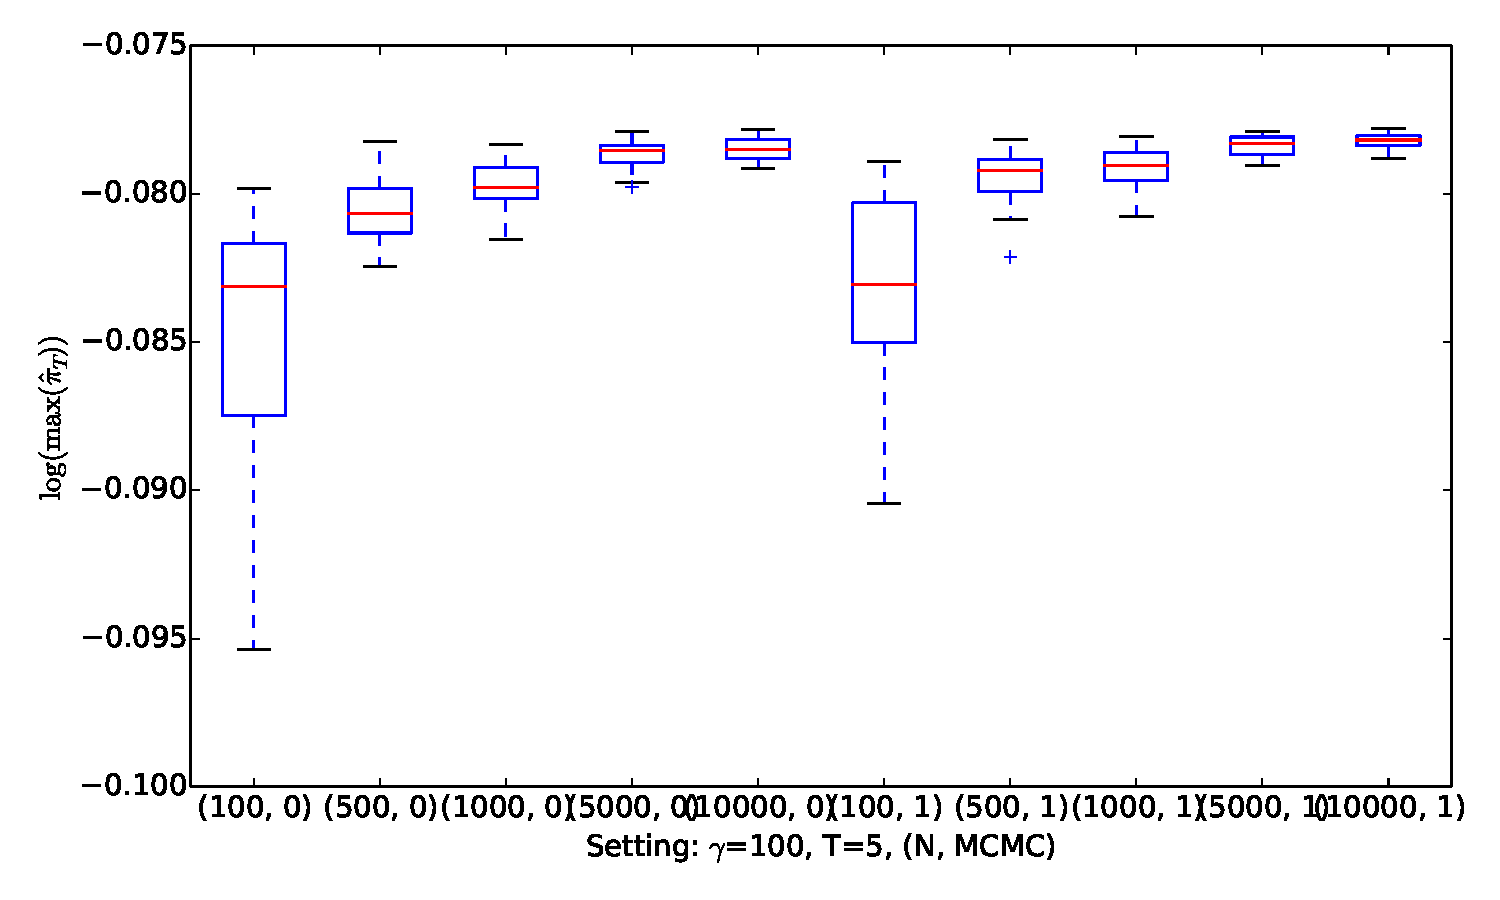
\includegraphics[width=\textwidth]{loglik_t_gs_n/T5_gamma100.pdf}
    \end{minipage}%
    \begin{minipage}{0.5\textwidth}
        \centering
        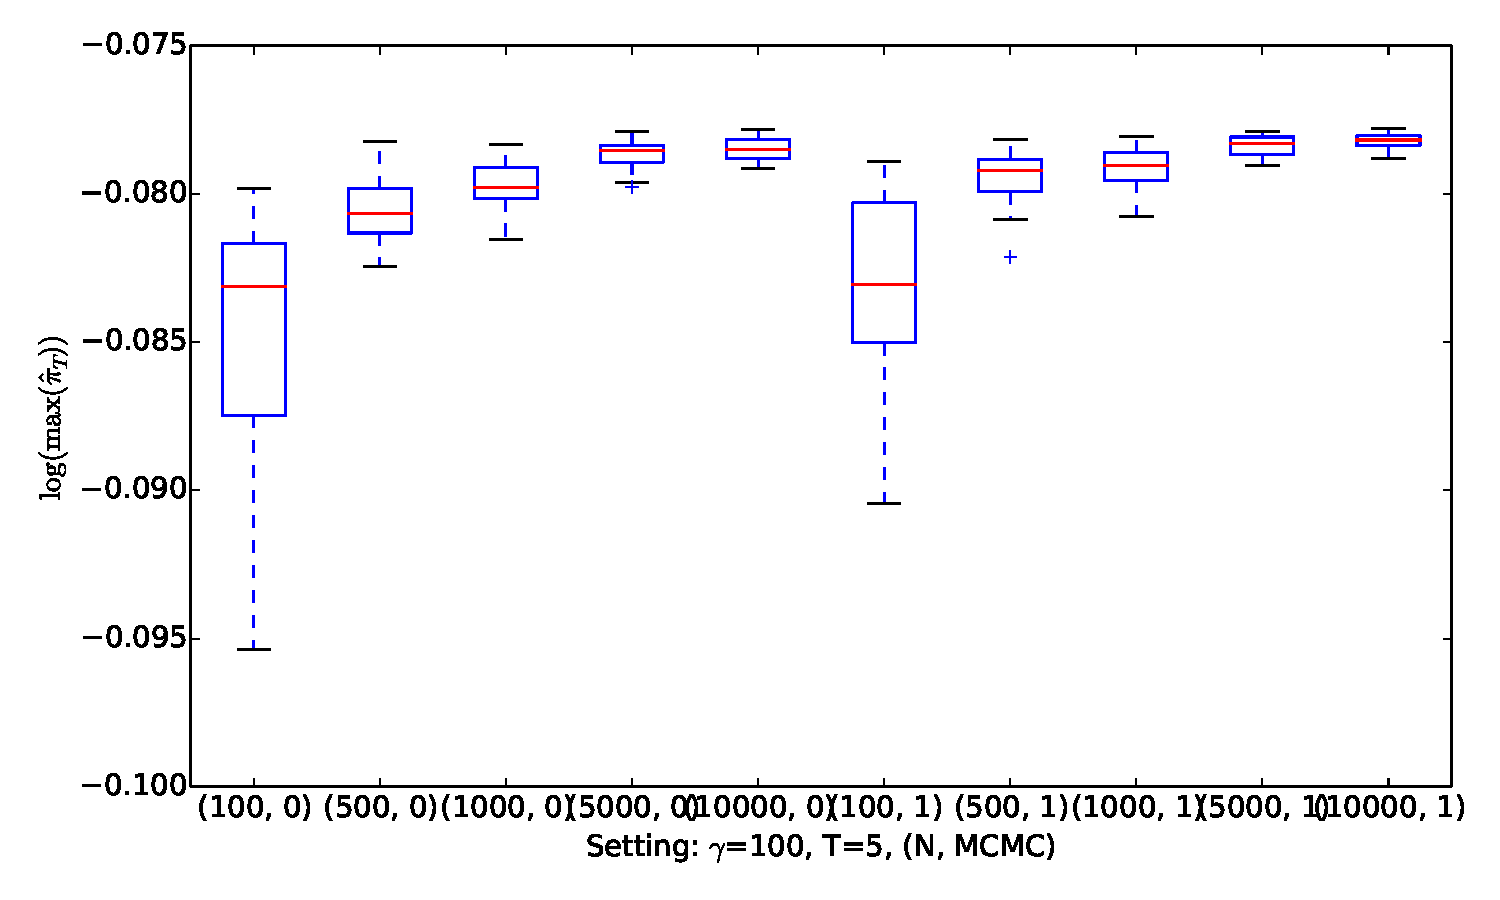
\includegraphics[width=\textwidth]{loglik_t_gs_n/T5_gamma100.pdf}
    \end{minipage}
    \caption{The $\log\pi_T(\hat{u}^*_{0:t})$ box-plots of 30 independent runs with four different $\gamma$s settings. The leftmost/rightmost $5$ box-plots in each figure are for the runs without/with resample-move step.}
    \label{fig:log}
\end{figure}

\begin{figure}[!htbp]
    \centering
    \begin{minipage}{.5\textwidth}
        \centering
        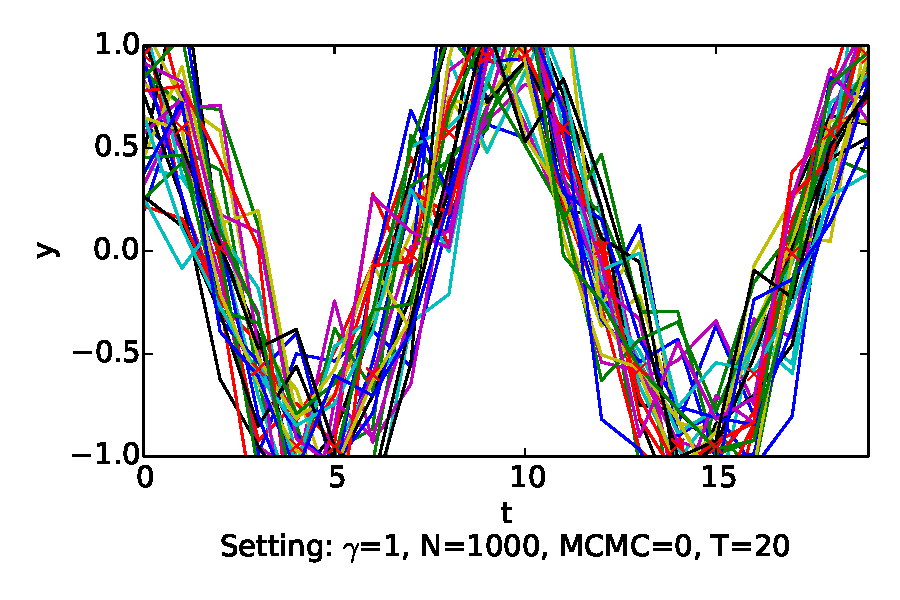
\includegraphics[width=\textwidth]{output_y/output_20_1.pdf}
        \caption*{$\gamma=1$}
    \end{minipage}%
    \begin{minipage}{0.5\textwidth}
        \centering
        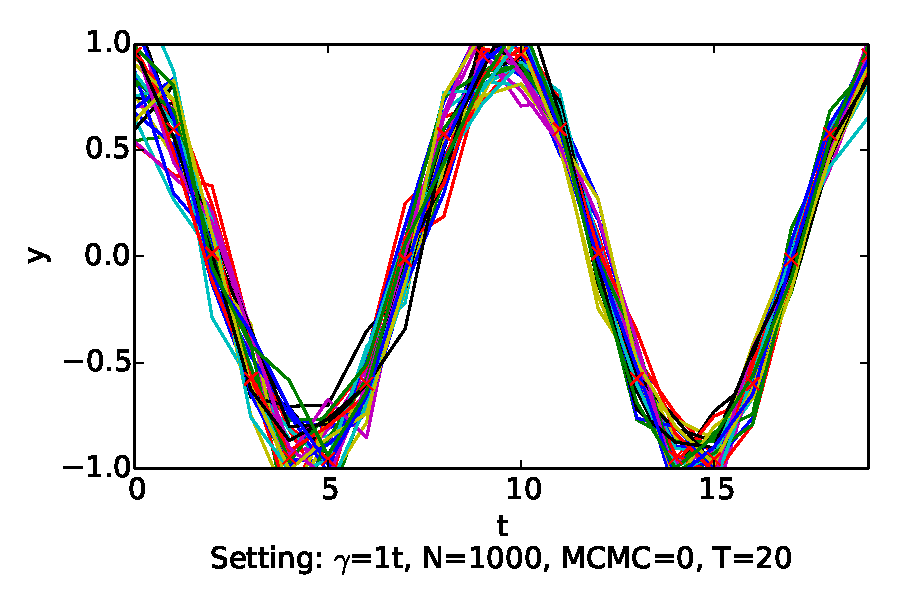
\includegraphics[width=\textwidth]{output_y/output_20_1t.pdf}
        \caption*{$\gamma=1t$}
    \end{minipage}
    \begin{minipage}{0.5\textwidth}
        \centering
        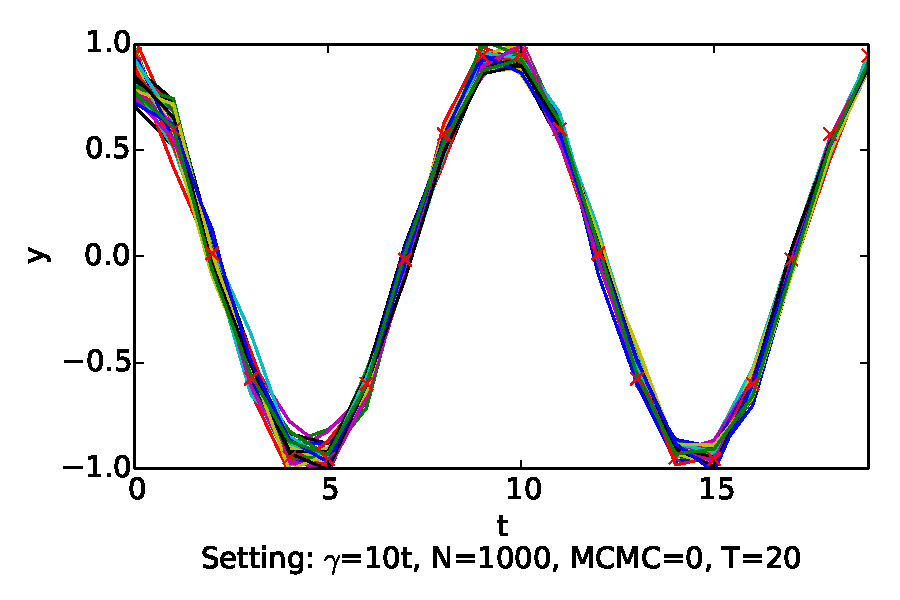
\includegraphics[width=\textwidth]{output_y/output_20_10t.pdf}
        \caption*{$\gamma=10t$}
    \end{minipage}%
    \begin{minipage}{0.5\textwidth}
        \centering
        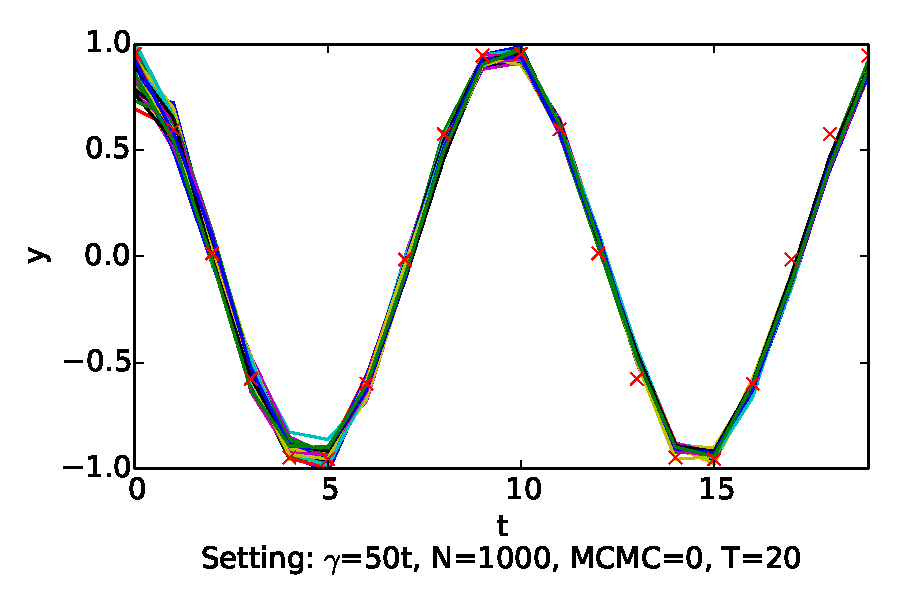
\includegraphics[width=\textwidth]{output_y/output_20_50t.pdf}
        \caption*{$\gamma=50t$}
    \end{minipage}
    \begin{minipage}{0.5\textwidth}
        \centering
        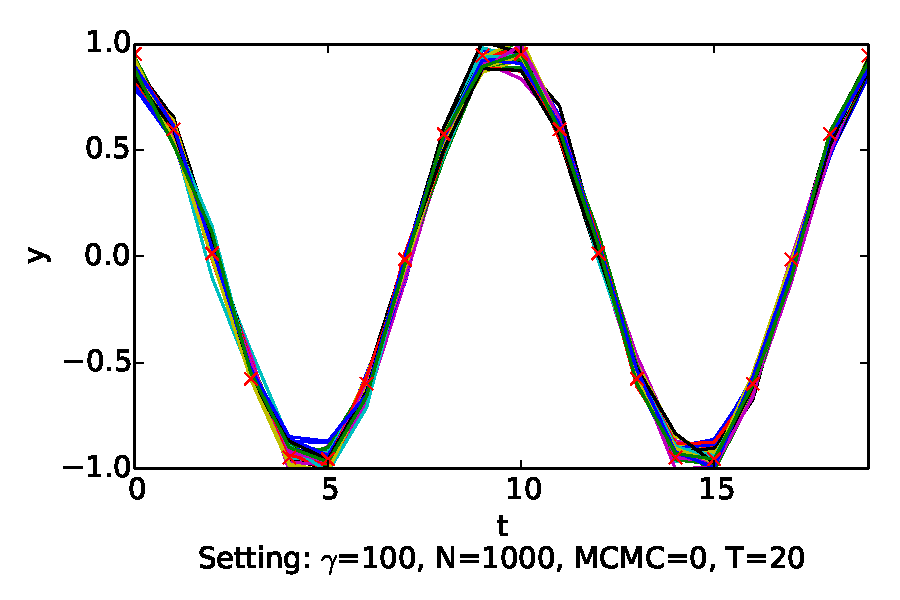
\includegraphics[width=\textwidth]{output_y/output_20_100.pdf}
        \caption*{$\gamma=100$}
    \end{minipage}%
    \begin{minipage}{0.5\textwidth}
        \centering
        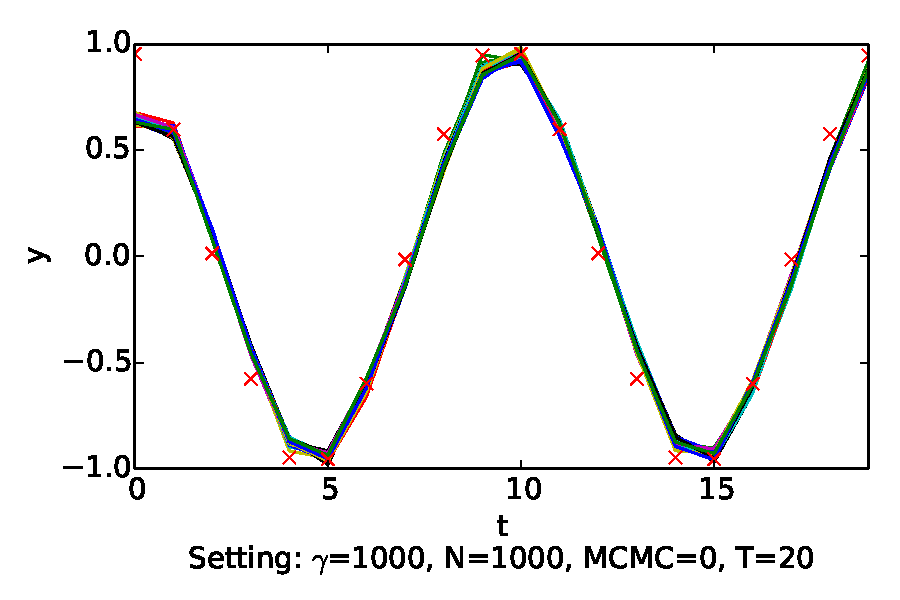
\includegraphics[width=\textwidth]{output_y/output_20_1000.pdf}
        \caption*{$\gamma=1000$}
    \end{minipage}
    \caption{The estimated $y$ output of the model using $u^*_{0:T}$ in 30 independent runs with various $\gamma$ settings, $T=20$, $N=1000$ and resample-move disabled.}
    \label{fig:estimatedy}
\end{figure}

\section{Example 2: Tracking the DAX Index}
\label{sec:exp2}
Given the initial result in Example 1 looks very promising, we attempt to investigate the use of the same algorithm to track the financial index using real-world data. We shall look at the German's DAX (Deutscher Aktienindex) Index, which consists of 30 German's blue chip stocks listed on Frankfurt Stock Exchange as the constituents from 1st January 2014 up to 30th June 2014. It represents $80\%$ of the aggregated prime standard's market capitalization. The DAX Index is chosen for various pragmatic reasons. It is one of the major world indices that is tracked by various index funds, it has small number of components and the data is freely accessible\footnote{Actually, we first looked at Dow Jones Industrial Average (DJIA) Index obtained. It was later found some of the data is not publicly available. Having said that, the preliminary findings concur with the findings we have with the DAX Index reported here.}. For further detail on the DAX Index methodology, refer \cite{DAX14}.
 
In the first experiment, we define a simple hypothetical sub-index, $DAX4$ consists of four stocks from the DAX Index that have the highest weights as of 2nd January 2014, namely Bayer (BAYN), Siemens (SIE), BASF (BAS) and Daimler (DAI). Then, the $DAX4$ index level is calculated as the simple weighted average of the adjusted close prices obtained from Yahoo Finance as follows:
\begin{equation}
  y = \sum_{s \in \mathcal{S}} w_s x_s
\end{equation}
where $y$ is the index level, $\mathcal{S}$ consists of the four stocks and  $w_s$ and $x_s$ are the weight and price of stock $s$ respectively. Here the weights of these four stocks are assigned to be $0.4$, $0.3$, $0.2$ and $0.1$ respectively. The adjusted close price of each stock along with the calculated index level are shown in Figure \ref{fig:adjclose}.
 
\begin{figure}[htbp]
\centering
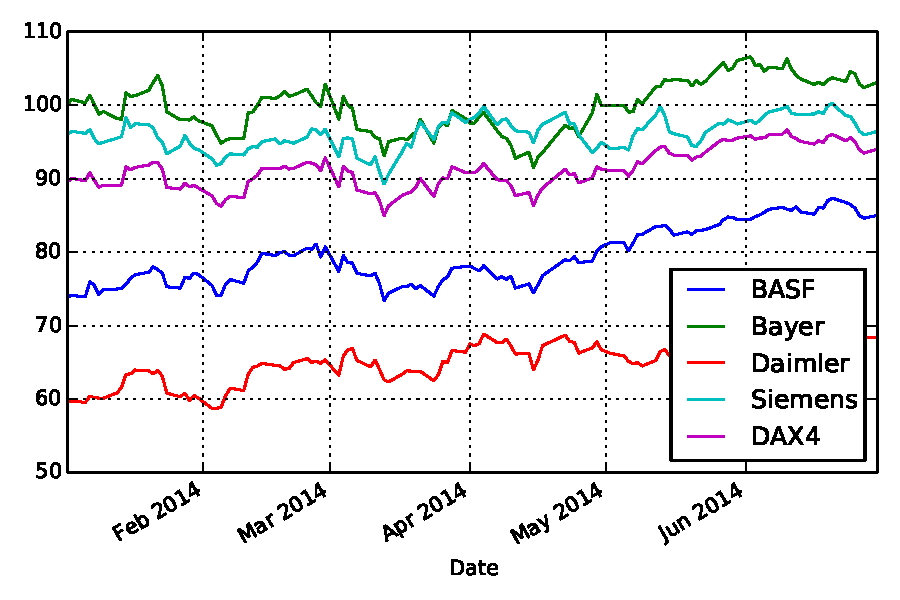
\includegraphics[width=\textwidth]{adjclose}
\caption{The adjusted close price of the 4 stocks and the calculated index level of $DAX4$.}
\label{fig:adjclose}
\end{figure}
 
The portfolio optimisation problem is formulated as such $y$ is viewed as the target reference level that a portfolio manager attempt to replicate as close as possible by changing the holding position on each component stocks in $\mathcal{S}$, at the same time, minimize the trasaction cost incurred in position changes.
 
To solve this problem using the SMC,  the following state space modelling is used:
\begin{align}
  X_t &= X_{t-1} + F_t(U_t) + \mu_{t_0} + \Sigma_{t_0} \\
  Y_t &= C_t(U_t)^{T}X_t
\end{align}
where $\{X_t\}_{t \geq 0}$ is a vector of stock price processes modelled as Arithmetic Brownian Motion with drift, $\{U_t\}_{t \geq 0}$ is a vector of control input processes, each represents the position we have for each stock, $F_t$ can be viewed as the market impact on price due to position changes, $\mu_{t_0}$ and $\Sigma_{t_0}$ are vector of the estimated mean and the estimated covariance matrix of the stock returns and $\{Y_t\}_{t \geq 0}$ is the process represents the index level. The values of $\mu_t$ and $\Sigma_t$ here are estimated using Exponential Weighted Moving Average (EWMA) approach with the decay rate, $\lambda$, set to $0.94$, which can be easily calculated in a recursion form as follows:
\begin{equation}
  P_t = \lambda P_{t-1} + (1-\lambda) Q_{t}
\end{equation}
where $P_t$ is the EWMA estimate and $Q_t$ is the new observation at time step $t$. It is obvious from these equations that the EWMA estimate at time $t$ depens on all the preceeding estimates at time $s$, where $s < t$. To ensure the quality of EWMA estimate, a 6 months warm up period is used, i.e., the EWMA estimate is calculated from 1st July 2013 onwards. The estimates of $\mu_{t_0}$ and $\Sigma_{t_0}$ obtained are as follows:
\begin{equation}
\mu_{t_0} =
\begin{blockarray}{c}
\\
\begin{block}{(c)}
~ 0.00049655 ~ \\
0.00215094 \\
0.00156870 \\
0.00203186 \\
\end{block}
\end{blockarray}
~\Sigma_{t_0} =
\begin{blockarray}{ccccc}
  BAYN & SIE & BAS & DAI & \\
\begin{block}{(cccc)c}
 ~ 0.00011122 & 0.00009616 & 0.00010233 & 0.00009828 ~ & BAYN \\
0.00009616 & 0.00013975 & 0.00010037 & 0.00008377 ~ & SIE \\
0.00010233 & 0.00010037 & 0.00014317 & 0.00010481 & BAS \\
0.00009828 & 0.00008377 & 0.00010481 & 0.00013398 & DAI \\
\end{block}
\end{blockarray}
\end{equation}
 
It is worth here to re-iterate here that this model is just a means to an end. There are more sophisticated models, e.g., Geometric Brownian Motion with drift, Jump diffusion model, etc.
 
Given the above model, we can write the reward function as follows:
\begin{equation}
  J(u_{1:T},y^{ref}_{1:T}, x_0) = \E_{x_0}\left[ -\dfrac{1}{2}\displaystyle\sum^T_{t=1}\left(\vert\vert y^{ref}_t - C_t(u_t)x_t - G_t(u_t) \vert\vert^2_{(D_t(u_t)D_t(u_t)^T)^{-1}}  + \vert\vert u_t - \Xi_t u_{t-1} \vert\vert^2_{L_t}\right) \right]
\end{equation}
 
For the state space model parameters we will use B = D = F = I and for the reward L1 = diag(0.1, 0.2, 0.3, 0.4) and L2 = diag(0.4, 0.3, 0.2, 0.1). Also, for the constraints of u2,n we have d1 = 2, d2 = 4, d3 = 6 and d4 = 8. The idea behind all choices is to construct a scenario where stations with with lower switching on/off cost are assigned higher “fuel” penalties (reflected upon higher values in L2) and more restrictive constraints on how much control power they can deliver (reflected upon dm). The reference is a one dimensional signal composed by a sequence of equally sized upward steps every 5 epochs up to some time before the middle of the horizon T, after which it decays with a sequence of equal but different than before downward steps.
 
This time, we will use the SMC algorithm to target $\pi^{\gamma_n}$ where $\gamma$ is a linearly increasing sequence chosen to be $\gamma=t$. This is a pragmatic compromise between accuracy and good mixing in the algorithm. For the importance sampling stepwe will propose for $U_{1,n}$ to either switch one station on, either shut one off, or keep the same configuration compared to U1,n−1. Each move is proposed with equal probability. For U2,n we will propose each time uniformly from U2. Simulations were carried out for N = 5000,10000,50000 without the MCMC moves implemented and the results are plotted in Figures 3 and 4. Given the difficulty to design MCMC moves with reasonable acceptance ratios for this model, the step was omitted. Instead to counter degeneracy it was chosen to use a large number of particles and a smoothly increasing γn . Simulations took less than a minute per 1000 particles.
The algorithm seems to perform well. We observed that in some simulation runs there seems to be a lag when the reference drops. We believe this is sensible with the problem’s parameter setting, which penalises in the same way turning on and shutting down a station and constraining Un,2 to be non-negative. So in some cases it is preferable to keep a station on with low output than switching it off. Improvements in terms of the accuracy of the mean of the recursive likelihood mn tracking the reference, or the smoothness or speed of the controllers can be always be achieved by different tuning for L1, L2, D.
 
\subsection{Result and discussion}
Various setting are attempted and repeated $n$ times, We tried and repeated couple of settings $T x L x $
 
The resulting $Y$ and $u$ are summaried in figure x.
 
As sho, we can see that the method is effective etc.
 
\subsection{Extension}
Tracking the full index, the results are shown here
 
\subsection{Partial Replication}
As discussed earlier, sometimes it may be more efficient in terms of cost to track the index with only a subset of its constituents. This can be achieved with minimal change on the model proposed, by doubling the number of stocks to be the top $8$ highest weighted constituents of DAX index as of 1st January 2014 and setting the the \emph{true} $DAX$ index level as the target reference $y$. The experiment is repeated as before and the results are shown in Figure .
 
\section{Model Control Predictive}
We demonstrate how the model control predictive can e used ot predict the value.Instead, we use this idea.
 
 
\subsection{Result}
 
\endinput
 
 
\section{Conclusions}
\label{sec:conclusion5}
This chapter presents some proof-of-concept experiments that have been
carried out to validate our proposal: inferring security policies from
decision examples using EAs. It first presents the experiments on
inferring some simple binary decision policies and continues with the
experiments on inferring the Fuzzy MLS model, which is a more
complicated multi-decision policy model. In all cases, the results
show that EAs are able to infer policies that can approximate (if not
refine) the original reference models that are used to generate the
training sets. The technique is also shown to be able to scale with
the range of input/output variables and to tolerate~``wrong'' examples
in the training set.
 
For a dynamic environment, the ability to infer policy from examples
alone is not sufficient. The inferred and learnt policies will
eventually become suboptimal over time as the operational requirements
change. The policy needs to be updated continually to maintain its
optimality. The next chapter demonstrates how multi-objective
evolutionary algorithms (MOEAs) can be used to achieve this goal.
